\section{Appendix}

\subsection{Evaluation Benchmarks}

\subsubsection*{Document Structure Tasks}

\begin{itemize}[
  leftmargin=1.0em,
  labelsep=0.5em
]
    \item \textbf{olmOCR-Bench}~\cite{poznanski2025olmocr} evaluates OCR and document parsing systems through simple, deterministic binary unit tests, analogous to software testing, enabling fair and transparent comparison across methods. It comprises 1,400 PDF pages and over 7,000 unit-test cases that span a broad range of document types and layout structures, providing a rigorous testbed for the robustness and generalization of document extraction systems.

    \item \textbf{ParseBench}~\cite{zhang2026parsebenchdocumentparsingbenchmark} targets document parsing for agentic workflows, emphasizing semantic correctness over surface text similarity. It contains roughly 2,000 human-verified pages from enterprise documents in insurance, finance, and government, organized along five capability dimensions: table structure, chart data, content faithfulness, semantic formatting, and visual grounding, each assessed with task-specific metrics. The benchmark therefore measures whether parsed outputs preserve the structure and meaning required for downstream automated decisions.

    \item \textbf{OmniDocBench}~\cite{ouyang2025omnidocbench} is a benchmark for comprehensive document parsing evaluation, with high-quality annotations across nine document sources ranging from academic papers and textbooks to more challenging handwritten notes and densely typeset newspapers. It supports multi-level evaluation, from end-to-end parsing to task-specific and attribute-level analysis, and covers 19 layout categories and 15 attribute labels for fine-grained comparison. Across this work we report three released versions of this benchmark: end-to-end document parsing uses OmniDocBench-v1.6, while the remaining evaluations use OmniDocBench-v1.5 and OmniDocBench-v1.0. These versions differ in document coverage and annotation refinements, so scores are comparable only within the same version.

    \item \textbf{DocLayNet}~\cite{pfitzmann2022doclaynet} is a large-scale benchmark for document layout analysis that addresses the limited layout diversity of earlier datasets. It provides over 80,000 manually annotated PDF pages from diverse sources, each labeled with bounding boxes across 11 layout categories, and includes a multiply annotated subset that establishes a human-agreement upper bound on performance.

    \item \textbf{D$^4$LA}~\cite{da2023vgt} is a dataset for document layout analysis covering 12 document categories and 27 layout types. It comprises 11,092 document images in total, of which 2,224 form the test set.

    \item \textbf{OmniDocBench Layout Subset}~\cite{ouyang2025omnidocbench} reuses the layout-region annotations of OmniDocBench-v1.5 to evaluate layout detection. Models predict bounding boxes for elements such as text, titles, tables, figures, and formulas, and accuracy is measured by mean intersection-over-union (mIoU) against the ground-truth regions.

\end{itemize}

\subsubsection*{Element-level Parsing Tasks}

\begin{itemize}[
  leftmargin=1.0em,
  labelsep=0.5em
]
    \item \textbf{OmniDocBench Text Subset}~\cite{ouyang2025omnidocbench} evaluates block-level text recognition. We crop all text-related regions from the 1,355 images of OmniDocBench-v1.5 according to their layout labels and discard null annotations, yielding 17,148 block-level images whose recognition quality is measured by edit distance similarity (EDS).

    \item \textbf{PubTabNet}~\cite{pubtabnet} is a large-scale benchmark for image-based table recognition, automatically built by aligning the XML and PDF representations of scientific articles from PubMed Central. It provides 500,777 training, 9,115 validation, and 9,138 test table images paired with structured HTML annotations of table structure and cell content. We evaluate on the validation split, measured by the Tree-Edit-Distance-based Similarity (TEDS) metric, which compares predicted and ground-truth tables as trees to jointly account for structural and content errors.

    \item \textbf{FinTabNet}~\cite{fintabnet} is a benchmark for table detection and cell-structure recognition in complex financial documents, drawn from the annual reports of S\&P 500 companies with HTML annotations of hierarchical cell structure. Its 112,887 tables are split into 91,596 training, 10,635 validation, and 10,656 test instances, and we evaluate on the validation split. It captures table styles that are common in practice yet underrepresented in scientific datasets.

    \item \textbf{UniMERNet}~\cite{wang2024unimernet} is a benchmark for mathematical expression recognition under real-world conditions. Its training set UniMER-1M offers over one million image-LaTeX pairs, while the evaluation set UniMER-Test contains 23,789 expressions across four categories: simple printed expressions (SPE), complex printed expressions (CPE), screen-capture expressions (SCE), and handwritten expressions (HWE).

    \item \textbf{ChartQA}~\cite{masry2022chartqa} is a chart-understanding benchmark of real-world charts, comprising 9.6K human-written and 23.1K machine-generated question-answer pairs that emphasize visual and arithmetic reasoning over chart content. In our evaluation it serves as the \textbf{Chart2Table} benchmark, where a model extracts the underlying data table from a chart image, scored by relative-mapping-similarity F1 (RMS-F1).

    \item \textbf{ChartX-SE}~\cite{chen2024onechart} is the structural-extraction split of the ChartX test set, used to evaluate \textbf{Chart2JSON} parsing on conventionally rendered bar, line, and pie charts. Models must recover the structured numerical content of each chart, evaluated by average precision at strict, slight, and high tolerance levels (AP@strict, AP@slight, AP@high).

    \item \textbf{ChartMimic~\cite{chartmimic}} is a \textbf{Chart2Code} generation benchmark that pairs 4,800 publication-style charts from scientific papers with the Python code that renders them, spanning 22 chart types and 201 subcategories. We evaluate on its Direct Mimic subset of 600 charts, reporting execution rate together with low-level scores (text, layout, type, and color) and a high-level visual-similarity score.

    \item \textbf{CoSyn-Chemical~\cite{cosyn}} is the chemical formula subset of CoSyn, a code-guided synthetic corpus in which images are rendered from programmatically generated code. Molecular structures are produced with RDKit alongside paired SMILES ground truth. We evaluate on its validation split of 128 image-text pairs, measuring optical chemical formula recognition by InChI exact-match accuracy, Tanimoto similarity, and valid SMILES rate.

    \item \textbf{ChemDraw-Bench} is an in-house business evaluation set for optical chemical formula recognition. It consists of roughly 200 challenging peptide and small-molecule SMILES sequences whose images are synthesized with the commercial software ChemDraw, probing generalization to realistic, publication-quality structures beyond synthetically rendered molecules. It adopts the same metrics as CoSyn-Chemical: InChI exact-match accuracy, Tanimoto similarity, and valid SMILES rate.

\end{itemize}

\subsubsection*{Reasoning and Generalization Tasks}

\begin{itemize}[
  leftmargin=1.0em,
  labelsep=0.5em
]
    \item \textbf{DocVQA}~\cite{docvqa} is a visual question answering benchmark over document images, comprising 39,463 training, 5,349 validation, and 5,188 test questions over 12,767 real industry-document images. We evaluate on the validation split. Answering requires jointly reading printed text and interpreting layout, tables, and figures, and is measured by average normalized Levenshtein similarity (ANLS).

    \item \textbf{InfoVQA}~\cite{infovqa} (InfographicVQA) is a visual question answering benchmark over infographics, comprising 23,946 training, 2,801 validation, and 3,288 test questions over 5,485 web-sourced images. We evaluate on the validation split. Its questions stress joint reasoning over text, graphical elements, and layout, frequently involving counting, sorting, and arithmetic, and are scored by ANLS.

    \item \textbf{AI2D}~\cite{kembhavi2016diagram} is a diagram-understanding benchmark built from over 5,000 grade-school science diagrams paired with more than 15,000 multiple-choice questions. It evaluates the ability to interpret diagrammatic elements such as labels, arrows, and icons together with their relationships, grounding language in structured visual layouts.

    \item \textbf{MathVista}~\cite{lu2023mathvista} is a benchmark for mathematical reasoning in visual contexts, aggregating 6,141 examples that pair figures, plots, and geometry diagrams with problems requiring both perception and multi-step reasoning. We evaluate on the testmini split of 1,000 examples. It stress-tests the full see-then-reason pipeline, where errors may stem from either visual extraction or symbolic computation.

    \item \textbf{MMBench}~\cite{liu2024mmbench} is a general-purpose benchmark for large vision-language models, with single-choice questions across 20 ability dimensions and parallel English and Chinese versions, split into 1,164 development and 1,784 test questions. We evaluate on the development split. It covers diverse question types, including recognition, attribute and relation reasoning, and OCR, under standardized prompts for fair cross-model comparison.

    \item \textbf{MMMU}~\cite{yue2024mmmu} is a benchmark for expert-level multimodal understanding, comprising 11.5K college-level questions across six disciplines, 30 subjects, and 30 image types such as charts, diagrams, maps, and chemical formulas. It emphasizes knowledge-intensive, reasoning-heavy problems that require integrating domain knowledge with visual evidence.

    \item \textbf{MMStar}~\cite{chen2024we} is a benchmark of 1,500 human-curated samples spanning six core capabilities and 18 detailed axes, designed to reduce visual redundancy and data leakage in existing evaluations. It offers a balanced testbed for fine-grained assessment of multimodal perception and reasoning.

    \item \textbf{OCRBench}~\cite{liu2024ocrbench} is a benchmark for OCR and text-centric visual understanding, consisting of 1,000 manually verified question-answer pairs across five tasks: text recognition, scene-text VQA, document-oriented VQA, key information extraction, and handwritten mathematical expression recognition. It assesses both accurate transcription and downstream comprehension of text in images.

\end{itemize}

\subsection{Evaluation Prompts}

To facilitate reproduction of our evaluation results, we provide the evaluation prompt for each task. By default, the \texttt{<image>} tag is prepended to the prompt text. For the reasoning and generalization tasks, we directly adopt the original prompts from the evaluation dataset.

\subsubsection*{Document Structure Tasks}

\begin{tcolorbox}[
  colback=gray!5,
  colframe=gray!60,
  title={Prompt for doc2json},
  fonttitle=\bfseries,
  breakable
]
\begin{lstlisting}[style=promptlisting, breakautoindent=false, breakindent=0pt]
- Extract layout information from the provided PDF image.
- For each layout element, output its bbox, category, and the text content within the bbox.
- Bbox format: [x1, y1, x2, y2].
- Allowed layout categories: ['header', 'title', 'text', 'figure', 'table', 'formula', 'figure_caption', 'table_caption', 'formula_caption', 'figure_footnote', 'table_footnote', 'page_footnote', 'footer'].
- Text extraction and formatting:
  1) For 'figure', the text field must be an empty string.
  2) For 'formula', format text as LaTeX.
  3) For 'table', format text as HTML.
  4) For all other categories (e.g., text, title), format text as Markdown.
- The output text must be exactly the original text from the image, with no translation or rewriting.
- Sort all layout elements in human reading order.
- Final output must be a single JSON object.
\end{lstlisting}
\end{tcolorbox}

\begin{tcolorbox}[
  colback=gray!5,
  colframe=gray!60,
  title={Prompt for doc2md},
  fonttitle=\bfseries,
  breakable
]
\begin{lstlisting}[style=promptlisting, breakautoindent=false, breakindent=0pt]
You are an AI assistant specialized in converting PDF images to Markdown format. Please follow these instructions for the conversion:

1. Text Processing:
- Accurately recognize all text content in the PDF image without guessing or inferring.
- Convert the recognized text into Markdown format.
- Maintain the original document structure, including headings, paragraphs, lists, etc.

2. Mathematical Formula Processing:
- Convert all mathematical formulas to LaTeX format.
- Enclose inline formulas with $ $. For example: This is an inline formula $E = mc^2$
- Enclose block formulas with $$ $$. For example: $$\\frac{-b \\pm \\sqrt{b^2 - 4ac}}{2a}$$

3. Table Processing:
- Convert tables to HTML format.

4. Figure Handling:
- Ignore figures content in the PDF image. Do not attempt to describe or convert images.

5. Output Format:
- Ensure the output Markdown document has a clear structure with appropriate line breaks between elements.
- For complex layouts, try to maintain the original document's structure and format as closely as possible.

Please strictly follow these guidelines to ensure accuracy and consistency in the conversion. Your task is to accurately convert the content of the PDF image into Markdown format without adding any extra explanations or comments.
\end{lstlisting}
\end{tcolorbox}

\begin{tcolorbox}[
  colback=gray!5,
  colframe=gray!60,
  title={Prompt for layout analysis},
  fonttitle=\bfseries,
  breakable
]
\begin{lstlisting}[style=promptlisting, breakautoindent=false, breakindent=0pt]
Please output the layout information from the PDF image, including each layout element's bbox and its category.
1. Bbox format: [x1, y1, x2, y2]
2. Layout Categories: ['header', 'title', 'text', 'figure', 'table', 'formula', 'figure_caption', 'table_caption', 'formula_caption', 'figure_footnote', 'table_footnote', 'page_footnote', 'footer']
3. Constraint: All layout elements must be sorted in human reading order.
4. Final Output: The entire output must be a single JSON object.
\end{lstlisting}
\end{tcolorbox}

\subsubsection*{Element-level Parsing Tasks}

\begin{tcolorbox}[
  colback=gray!5,
  colframe=gray!60,
  title={Prompt for table2html},
  fonttitle=\bfseries,
  breakable
]
\textbf{Randomly select any one of the following prompts:} \\
\begin{lstlisting}[style=promptlisting, breakautoindent=false, breakindent=0pt]
1. Please encode the table from the image into HTML format.
2. Convert the table found in the image into HTML format.
3. Render the table in the image as HTML code, please.
4. Examine the table in the provided image and generate an HTML text representation of the table.
5. Watch this table and show an HTML-style reconstructed table in text. Only preserve the basic table structure and content.
\end{lstlisting}
\end{tcolorbox}

\begin{tcolorbox}[
  colback=gray!5,
  colframe=gray!60,
  title={Prompt for table2md},
  fonttitle=\bfseries,
  breakable
]
\textbf{Randomly select any one of the following prompts:} \\
\begin{lstlisting}[style=promptlisting, breakautoindent=false, breakindent=0pt]
1. Convert the table found in the image into Markdown format.  
2. Please encode the table from the image into Markdown format.  
3. Transform the image's table into the Markdown format, please.  
4. Render the table in the image as Markdown code, please.  
5. Convert the image's table data into the Markdown structure.  
\end{lstlisting}
\end{tcolorbox}

\begin{tcolorbox}[
  colback=gray!5,
  colframe=gray!60,
  title={Prompt for formula2latex},
  fonttitle=\bfseries,
  breakable
]
\textbf{Randomly select any one of the following prompts:} \\
\begin{lstlisting}[style=promptlisting, breakautoindent=false, breakindent=0pt]
1. Convert formulas in images to LaTeX format.
2. Convert the equations found in the images into LaTeX format.
3. Transform the formulas in images into LaTeX format, please.
4. Render the formulas in images as LaTeX equations, please.
5. Please transcribe the formulas from images into LaTeX format.
\end{lstlisting}
\end{tcolorbox}

\begin{tcolorbox}[
  colback=gray!5,
  colframe=gray!60,
  title={Prompt for chart2table},
  fonttitle=\bfseries,
  breakable
]
\textbf{Randomly select any one of the following prompts:} \\
\begin{lstlisting}[style=promptlisting, breakautoindent=false, breakindent=0pt]
[Option1]
You are an expert data analyst. Your task is to extract data from the provided chart image and strictly convert it into a plain Markdown table format.

[Option2]
Observe the following strict rules:
1. Headers: Use the actual chart title, legend, or axis labels as column headers. DO NOT use generic headers like "Characteristic" or "Value".
2. Values: Extract the exact raw numerical values. DO NOT append units (like %) or years to the data cells if they are already described in the headers.
3. Format: Use standard Markdown table syntax with `|` to separate columns, including a separator row (e.g., `|---|---|`). Ensure every line starts and ends with the `|` character.
4. Output: Provide ONLY the table. Do not include any introductory text, concluding remarks, or repetitions. STOP generating immediately after the last row of the table.

### Example 1
User: <image>
please convert the image to a markdown table

Assistant:
| Entity | 1991 | 1995 | 2000 | 2005 | 2010 | 2015 | 2017 |
|---|---|---|---|---|---|---|---|
| Mongolia | 46.867000579834 | 54.5810012817383 | 53.0040016174316 | 45.6650009155273 | 33.5270004272461 | 28.4529991149902 | 30.4220008850098 |

### Current Task
User: <image>
please convert the image to a markdown table

Assistant:
\end{lstlisting}
\end{tcolorbox}

\begin{tcolorbox}[
  colback=gray!5,
  colframe=gray!60,
  title={Prompt for chart2json},
  fonttitle=\bfseries,
  breakable
]
\textbf{Randomly select any one of the following prompts:} \\
\begin{lstlisting}[style=promptlisting, breakautoindent=false, breakindent=0pt]
1. You are an expert at analyzing charts and extracting their key information into a structured JSON format.
2. Act as a chart analysis expert: analyze charts, distill key insights, and deliver them as structured JSON.
3. You're great at reading charts-grab the essentials and put them into clean, structured JSON.
4. Role: Chart analysis specialist. Responsibilities: chart parsing; key info extraction; output: structured JSON.
5. I need you to analyze charts like an expert and output the key information in structured JSON.
\end{lstlisting}
\end{tcolorbox}

\begin{tcolorbox}[
  colback=gray!5,
  colframe=gray!60,
  title={Prompt for chart2code},
  fonttitle=\bfseries,
  breakable
]
\begin{lstlisting}[style=promptlisting, breakautoindent=false, breakindent=0pt]
You are an expert Python developer who specializes in writing matplotlib code based on a given picture. I need your help to generate the Python code that can reproduce the picture based on the picture I provide. Now, please give me the matplotlib code that reproduces the picture.
\end{lstlisting}
\end{tcolorbox}

\begin{tcolorbox}[
  colback=gray!5,
  colframe=gray!60,
  title={Prompt for chem2smiles},
  fonttitle=\bfseries,
  breakable
]
\textbf{Randomly select any one of the following prompts:} \\
\begin{lstlisting}[style=promptlisting, breakautoindent=false, breakindent=0pt]
1. Please convert this chemical structure to its SMILES string representation.
2. Convert the chemical structure shown to standard SMILES notation.
3. Generate the SMILES string for the chemical structure displayed in the image.
4. What is the SMILES representation of the chemical compound shown?
5. Convert all chemical diagrams in the image to their SMILES format and separate them with newlines.
\end{lstlisting}
\end{tcolorbox}

\subsection{Financial Information Extraction: Task Definition and Pipeline}
\label{appendix:fie}

This appendix details the Financial Information Extraction (FinIE) task used as a downstream evaluation of Infinity-Parser2 (Table~\ref{tab:finie}). Annual reports, drawn primarily from the stock market in our benchmark, represent a challenging domain for document intelligence: a single report often spans several hundred pages and couples frameless, multi-column layouts with a high density of tabular data. Our task targets the three primary statements, the balance sheet, the income statement, and the cash flow statement, which the pipeline must first locate and then transcribe in full with high structural fidelity.

\subsubsection*{Task Definition}
The objective of FinIE is to extract the three primary financial statements, the balance sheet, the income statement, and the cash flow statement, in their entirety from an unstructured PDF report. Rather than querying individual indicators, the task transcribes every line item of each primary statement in a single pass. Note references are recorded verbatim but not expanded, so the detailed note tables are left untouched. We formulate it as a structured extraction task with the following inputs and outputs.

\begin{tcolorbox}[
  colback=gray!5,
  colframe=gray!60,
  title={Definition of FinIE},
  fonttitle=\bfseries,
  breakable
]
\textbf{Input:} \\
\begin{enumerate}[
  leftmargin=1.0em,
  labelsep=0.5em
]
\item PDF Document $\mathcal{D}$.
\item Extraction directive $\mathcal{I}$: extract the balance sheet, the income statement, and the cash flow statement, without expanding note references.
\end{enumerate}

\medskip
\textbf{Output:} A JSON object with one entry per primary statement. Each entry carries the statement name, its reporting \texttt{periods} (given as \texttt{cutoff\_date}s) and their \texttt{period\_type}, the reporting \texttt{currency} and \texttt{unit}, and an array of line-item records. Each record holds the source \texttt{page}, the original line-item label, the amounts for the current and prior periods (\texttt{amount\_cy}, \texttt{amount\_py}), and the unexpanded \texttt{notes} reference.
\end{tcolorbox}

\subsubsection*{Parse-Locate-Extract Pipeline}
Processing an entire annual report at once is infeasible, given context-window limits and the noise introduced by hundreds of irrelevant pages. We therefore adopt a modular pipeline with three stages: full-document parsing, three-statement page localization, and LLM-based statement extraction with intra-statement validation. To isolate the contribution of document parsing, we fix the localization and extraction modules and vary only the parser, so that any change in end-to-end accuracy is attributable to parsing quality.

\begin{itemize}[
  leftmargin=1.0em,
  labelsep=0.5em
]
    \item \textbf{Stage 1: Full-Document Parsing.} Each page of the raw PDF is converted into structured text by the candidate parser, namely Infinity-Parser2-Flash*, MinerU2.5~\cite{niu2025mineru2}, PaddleOCR-VL-1.5~\cite{cui2025paddleocr}, or DeepSeek-OCR-2~\cite{wei2026deepseek2}. Tables are serialized to HTML and running text to Markdown, while element coordinates and reading order are preserved. This stage is decisive: a single merged cell or a broken reading order corrupts the data irrecoverably and propagates to every later stage.

    \item \textbf{Stage 2: Three-Statement Page Localization.} Because the target line items reside almost entirely in the balance sheet, the income statement, and the cash flow statement, we locate the pages of these three statements rather than scan the whole report. We combine complementary localization signals, principally keyword search and RAG-based semantic search. Keyword search matches canonical statement headings and their bilingual variants (for example, ``Consolidated Balance Sheet'' or its Chinese equivalent) against the parsed text to nominate candidate pages. RAG-based semantic search then embeds each parsed page and the canonical descriptions of the three statements with Inf-Retriever-v1~\cite{infly-ai_2025} and ranks pages by semantic similarity, recovering statements whose headings are abbreviated or missing. The candidate sets are merged and deduplicated to yield the located statement pages, whose parsed content forms the context $\mathcal{C}$.

    \item \textbf{Stage 3: LLM-based Statement Extraction and Validation.} The context $\mathcal{C}$ is passed to DeepSeek-V4-Flash~\cite{deepseekai2026deepseekv4}, a large language model prompted to transcribe every line item of the three primary statements into the structured JSON defined above. Note references are copied verbatim without expansion, and consistency checks are performed within each primary statement, verifying that subtotals reconcile with their component rows and that the balance-sheet identity holds, with total assets equal to the sum of total liabilities, mezzanine equity, and total equity. Operating on the localized statement pages rather than the full report keeps the input within the context window and suppresses spurious matches from unrelated sections.
\end{itemize}

\subsubsection*{Example Output}
Applying the pipeline to a representative annual report (amounts in RMB millions) yields, for each primary statement, an array of line-item records. An abridged excerpt appears below. The two amount columns correspond to the current and prior periods declared in \texttt{periods}, and the \texttt{notes} reference is retained verbatim without expansion.

\begin{tcolorbox}[
  colback=gray!5,
  colframe=gray!60,
  title={Example FinIE Output},
  fonttitle=\bfseries,
  breakable
]
\begin{lstlisting}[basicstyle=\ttfamily\small, breaklines=true]
{
  "balance_sheet": {
    "statement": "Consolidated Balance Sheet",
    "period_type": "as_of",
    "periods": ["20240331", "20230331"],
    "currency": "RMB",
    "unit": "million",
    "line_items": [
      {"page": 256, "line_item": "Cash and cash equivalents", "amount_cy": "248,125", "amount_py": "193,086", "notes": "Note 2(p)"},
      {"page": 256, "line_item": "Total current assets", "amount_cy": "752,864", "amount_py": "697,966", "notes": null},
      {"page": 256, "line_item": "Total assets", "amount_cy": "1,764,829", "amount_py": "1,753,044", "notes": null},
      {"page": 257, "line_item": "Total liabilities, mezzanine equity and equity", "amount_cy": "1,764,829", "amount_py": "1,753,044", "notes": null}
    ]
  },
  "income_statement": {
    "statement": "Consolidated Income Statement",
    "period_type": "year_ended",
    "periods": ["20240331", "20230331"],
    "currency": "RMB",
    "unit": "million",
    "line_items": [
      {"page": 254, "line_item": "Revenue", "amount_cy": "941,168", "amount_py": "868,687", "notes": "Note 5, 22"},
      {"page": 254, "line_item": "Income from operations", "amount_cy": "113,350", "amount_py": "100,351", "notes": null},
      {"page": 254, "line_item": "Net income", "amount_cy": "71,332", "amount_py": "65,573", "notes": null}
    ]
  },
  "cash_flow_statement": {
    "statement": "Consolidated Cash Flow Statement",
    "period_type": "year_ended",
    "periods": ["20240331", "20230331"],
    "currency": "RMB",
    "unit": "million",
    "line_items": [
      {"page": 261, "line_item": "Net cash provided by operating activities", "amount_cy": "182,593", "amount_py": "199,752", "notes": null},
      {"page": 263, "line_item": "Cash and cash equivalents, restricted cash and escrow receivables at end of year", "amount_cy": "286,424", "amount_py": "229,510", "notes": null}
    ]
  }
}
\end{lstlisting}
\end{tcolorbox}

\subsection{Visualization Results}

\begin{figure*}[htbp]
    \centering
    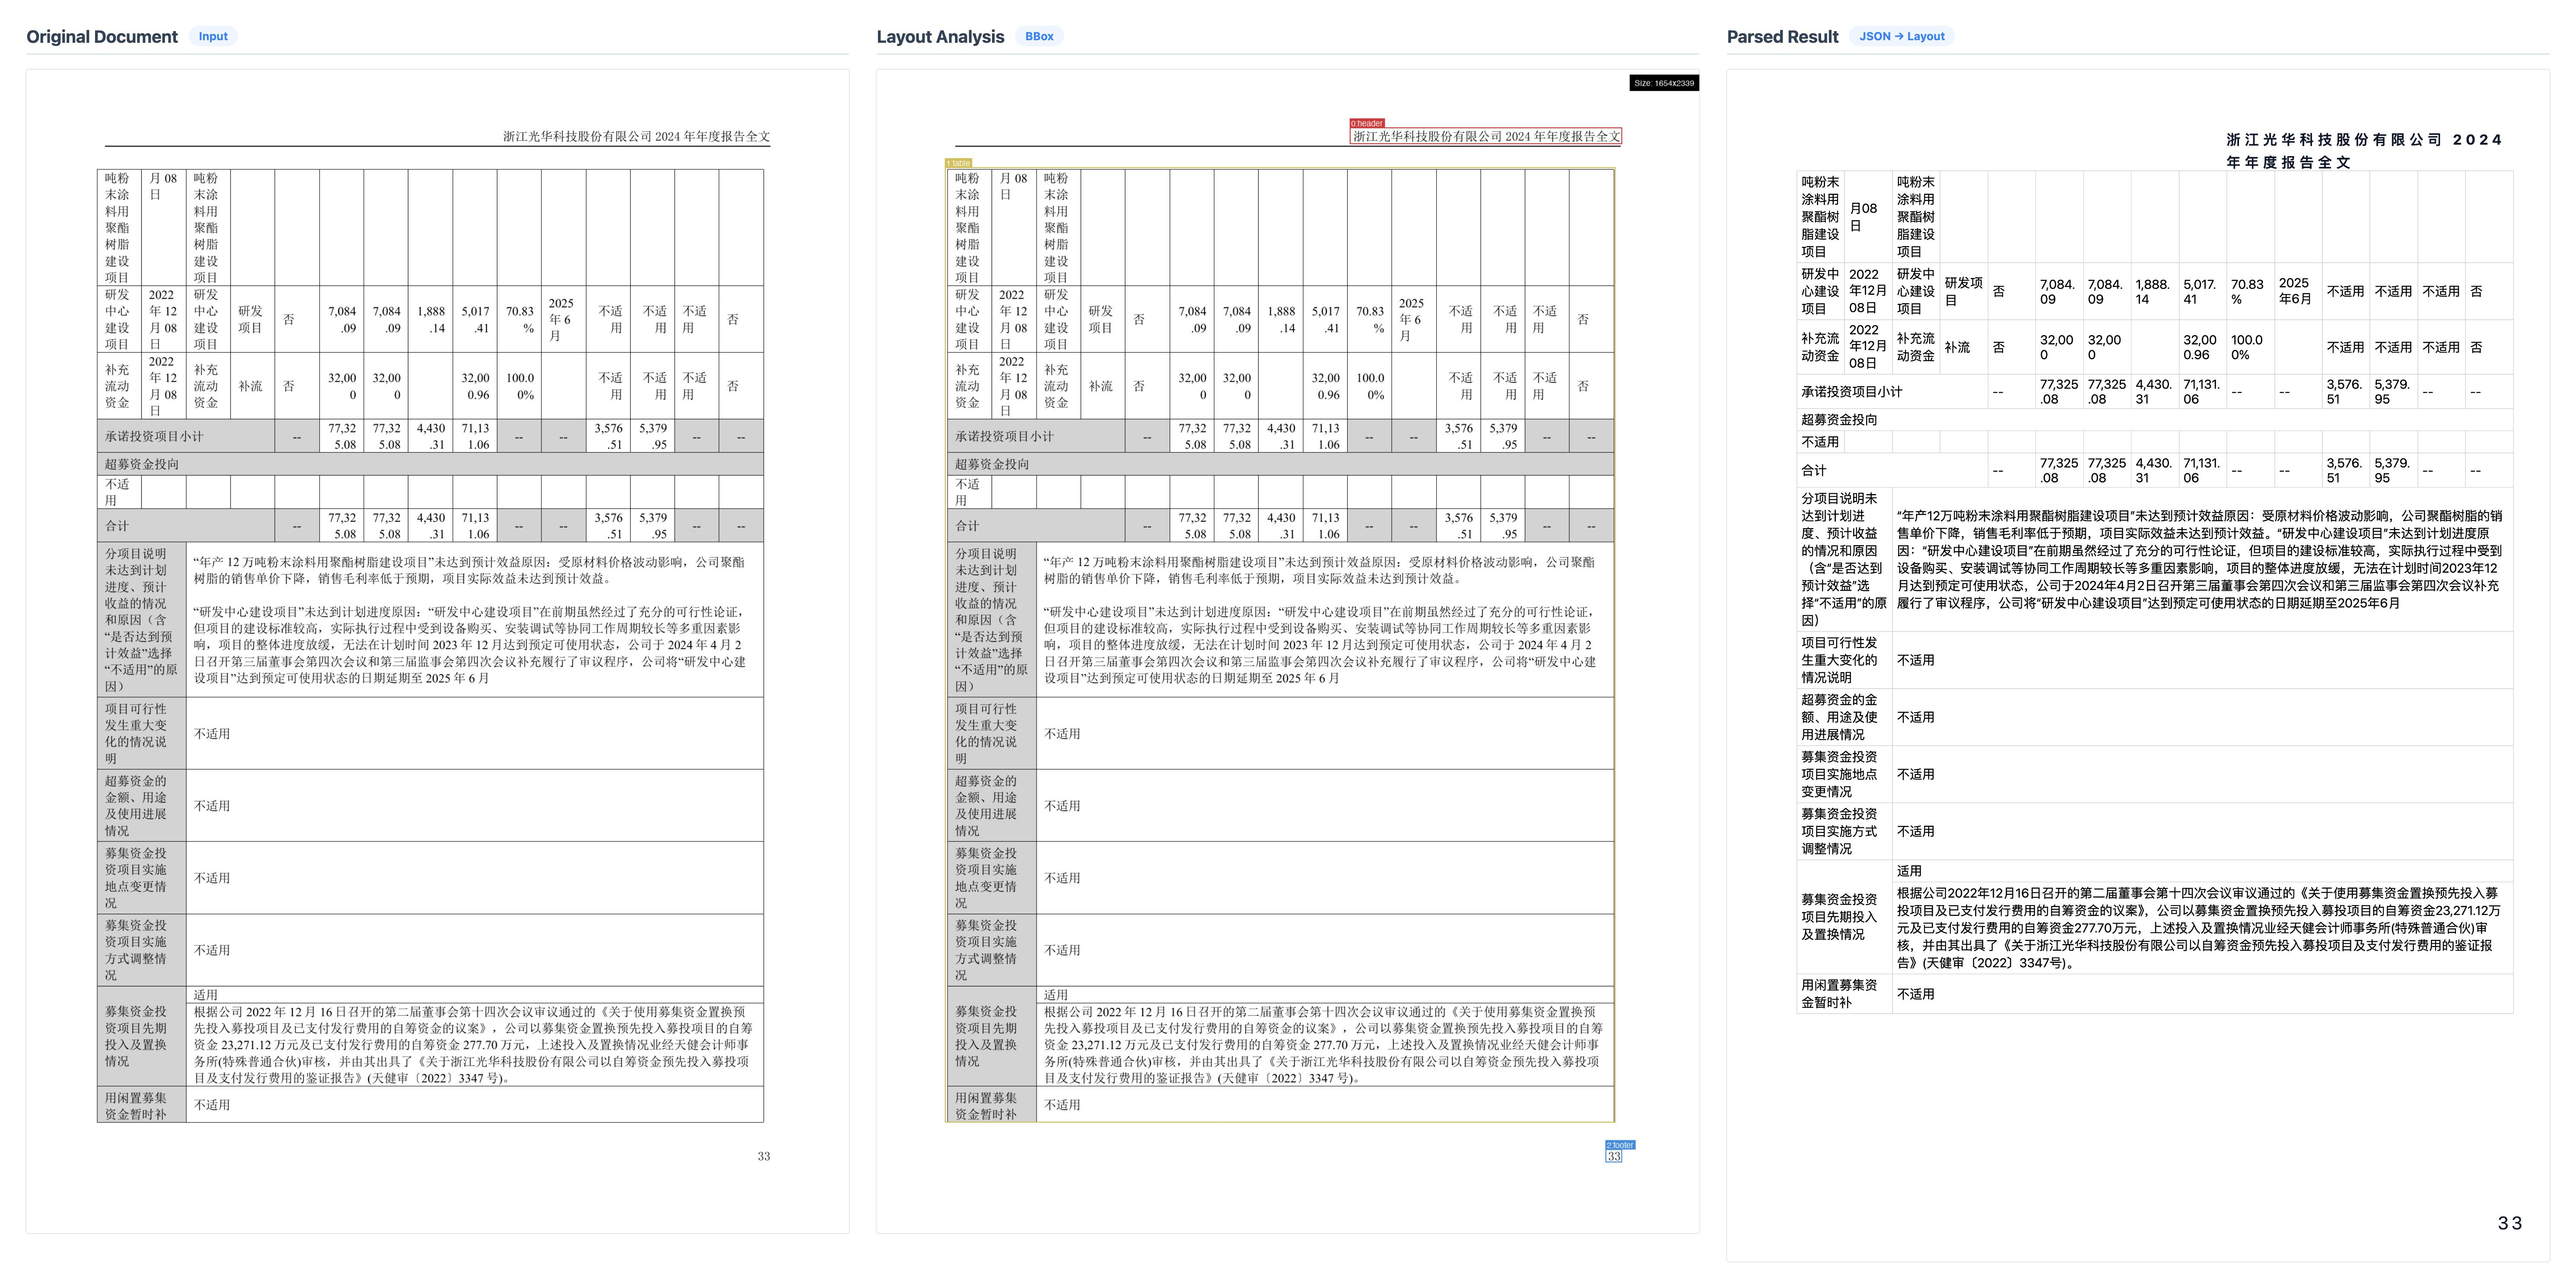
\includegraphics[width=\textwidth]{figures/visualization_results_a_stock.pdf}
    \caption{Visualization results of the A-stock image. The challenge is accurately determining column spans (colspans) in tables to prevent miscounting.}
    \label{fig:visualization_results_a_stock}
\end{figure*}

\begin{figure*}[htbp]
    \centering
    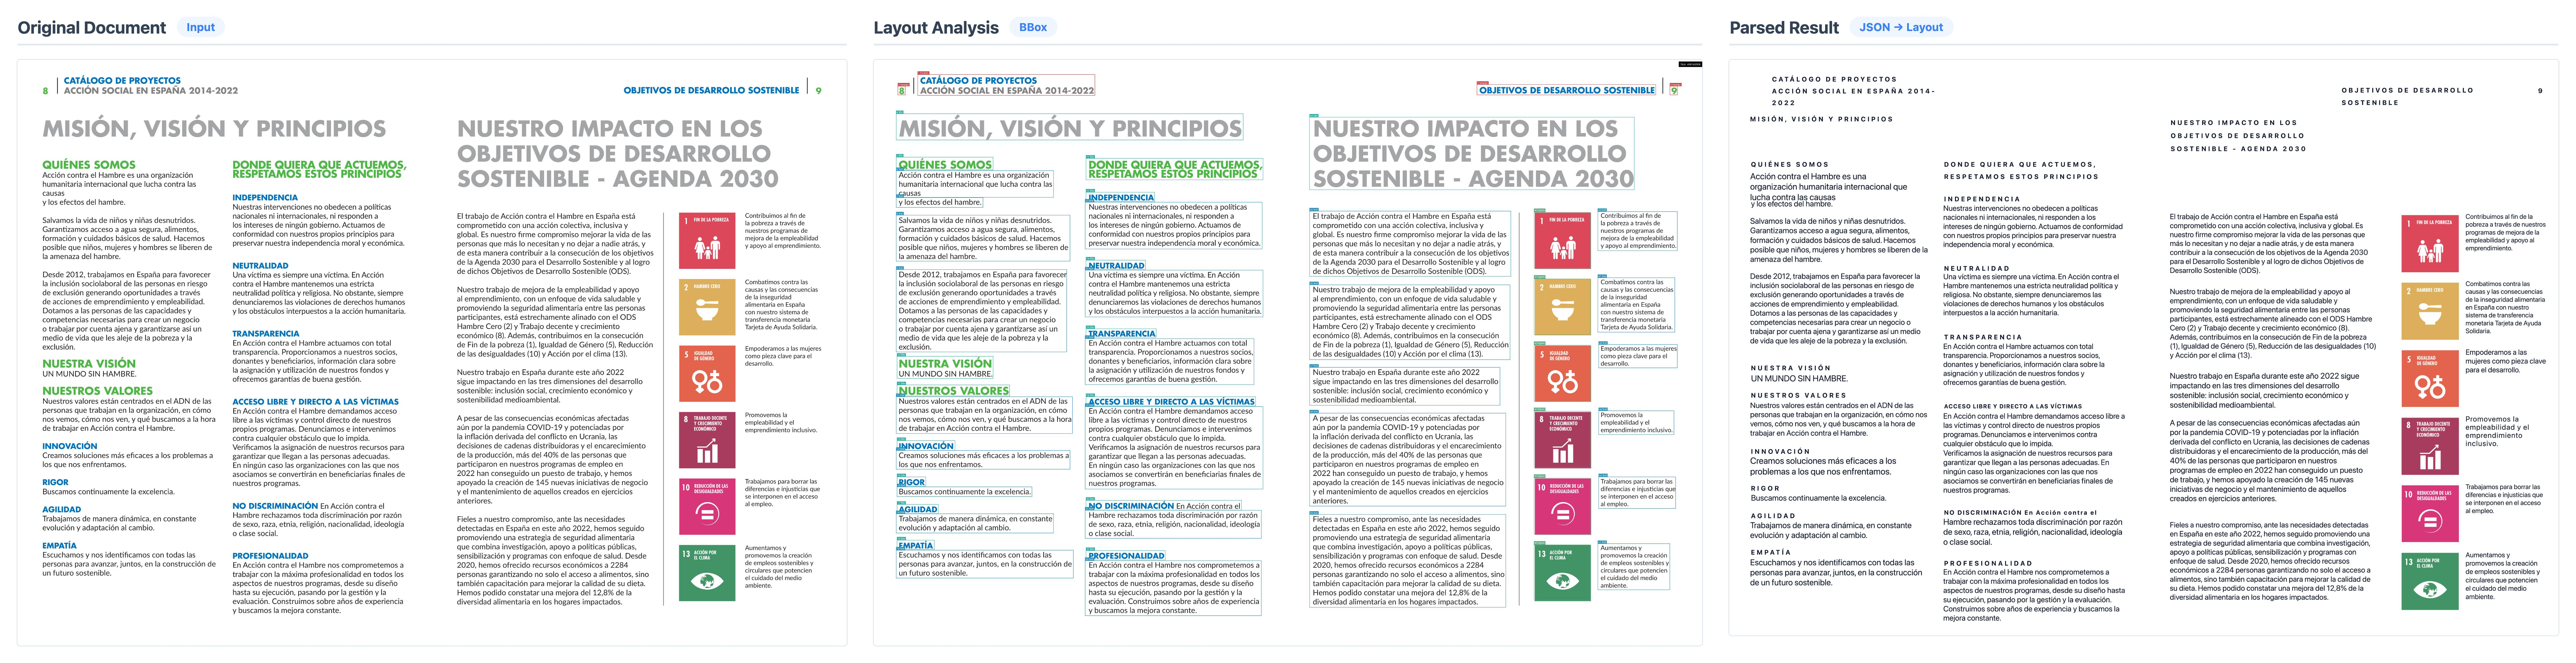
\includegraphics[width=\textwidth]{figures/visualization_results_muti_column.pdf}
    \caption{Visualization results of the multi-column image. The difficulty lies in executing complex layout analysis and accurately recovering the reading order.}
    \label{fig:visualization_results_muti_column}
\end{figure*}

\begin{figure*}[htbp]
    \centering
    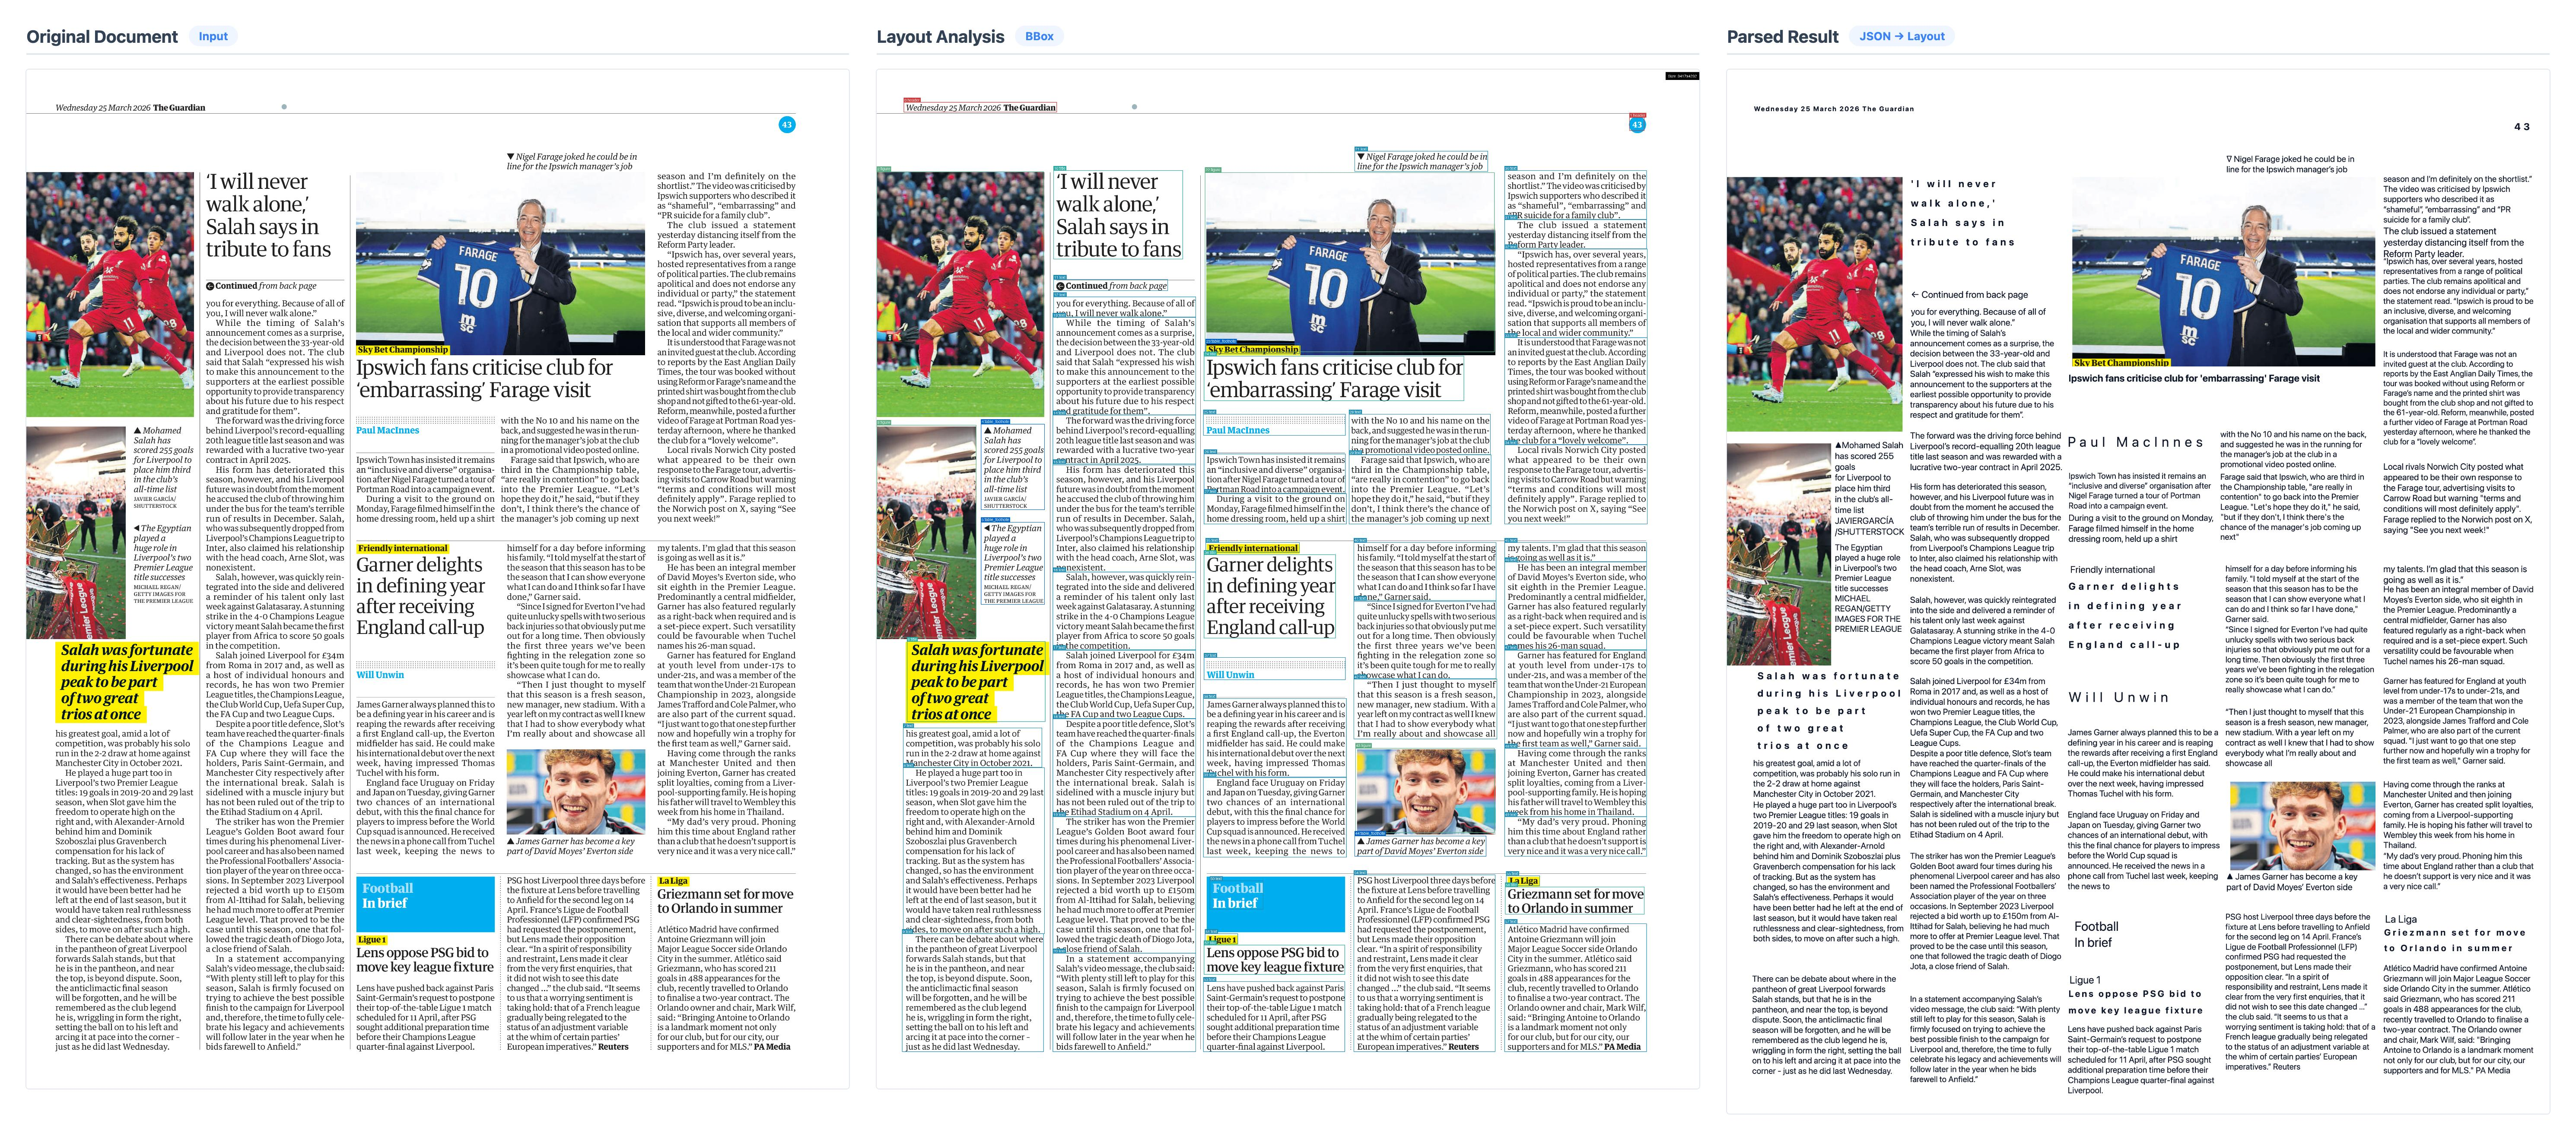
\includegraphics[width=\textwidth]{figures/visualization_results_newspaper_1.pdf}
    \caption{Visualization results of the newspaper image. The primary challenge is avoiding bounding box omissions caused by ultra-dense text distribution, narrow column margins, and microscopic fonts.}
    \label{fig:visualization_results_newspaper_1}
\end{figure*}

\begin{figure*}[htbp]
    \centering
    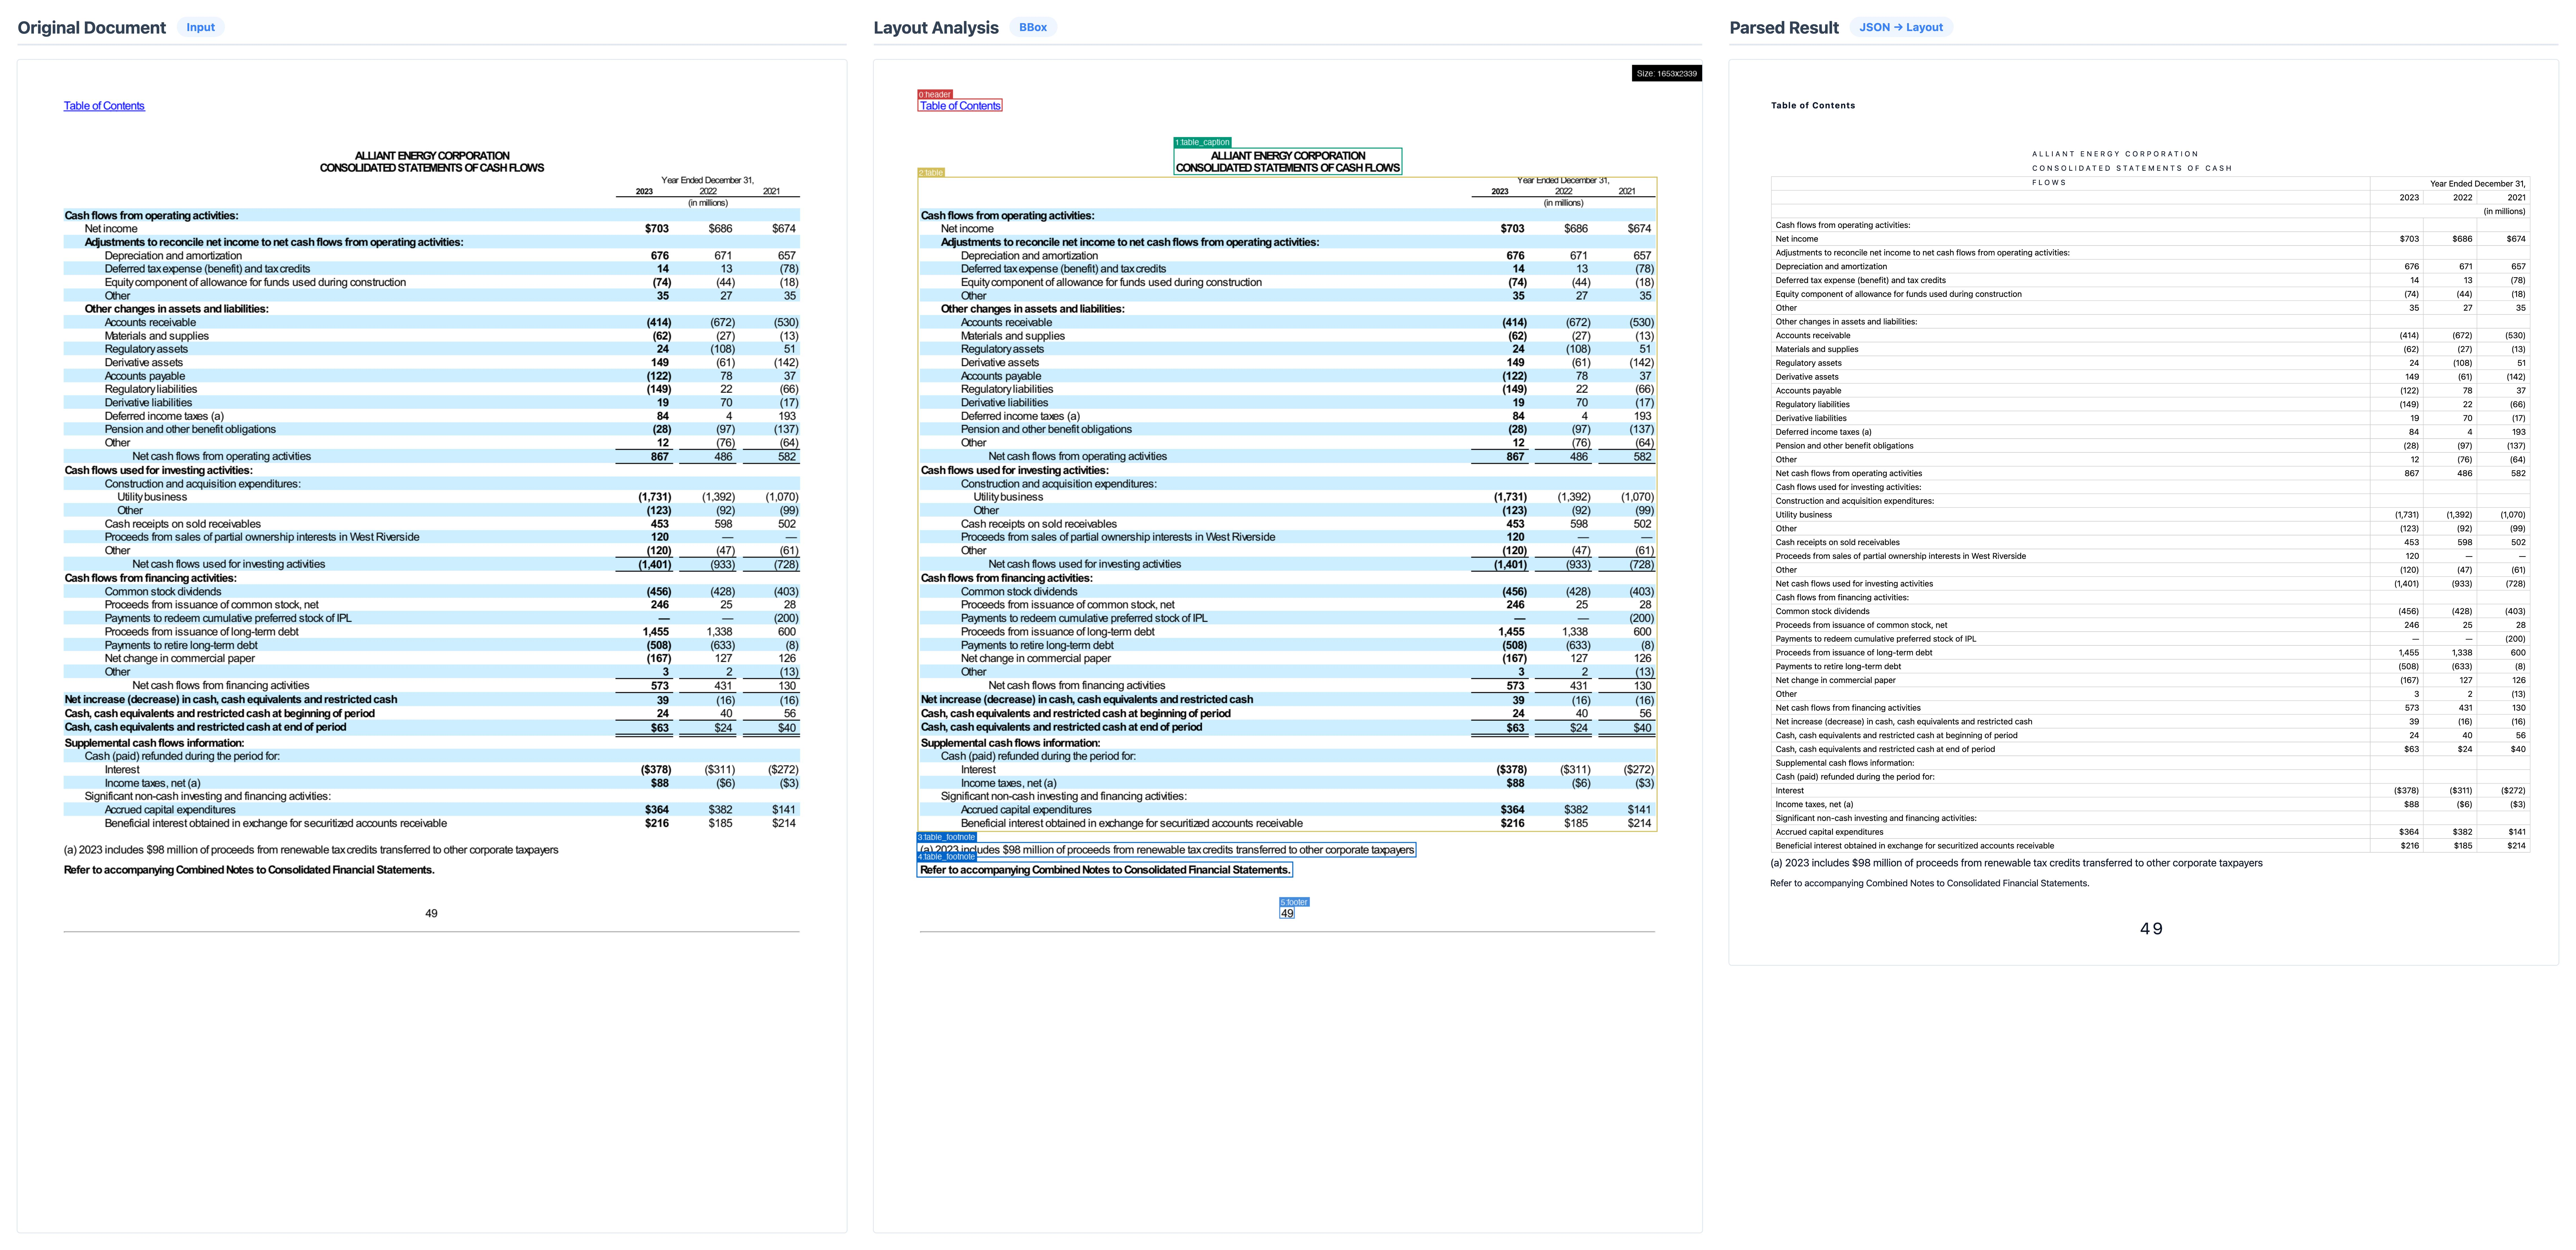
\includegraphics[width=\textwidth]{figures/visualization_results_us_stock.pdf}
    \caption{Visualization results of the US-stock image. The difficulty involves achieving precise row alignment across wide frameless spaces and capturing the hierarchical semantics of indented headers.}
    \label{fig:visualization_results_us_stock}
\end{figure*}

\begin{figure*}[htbp]
    \centering
    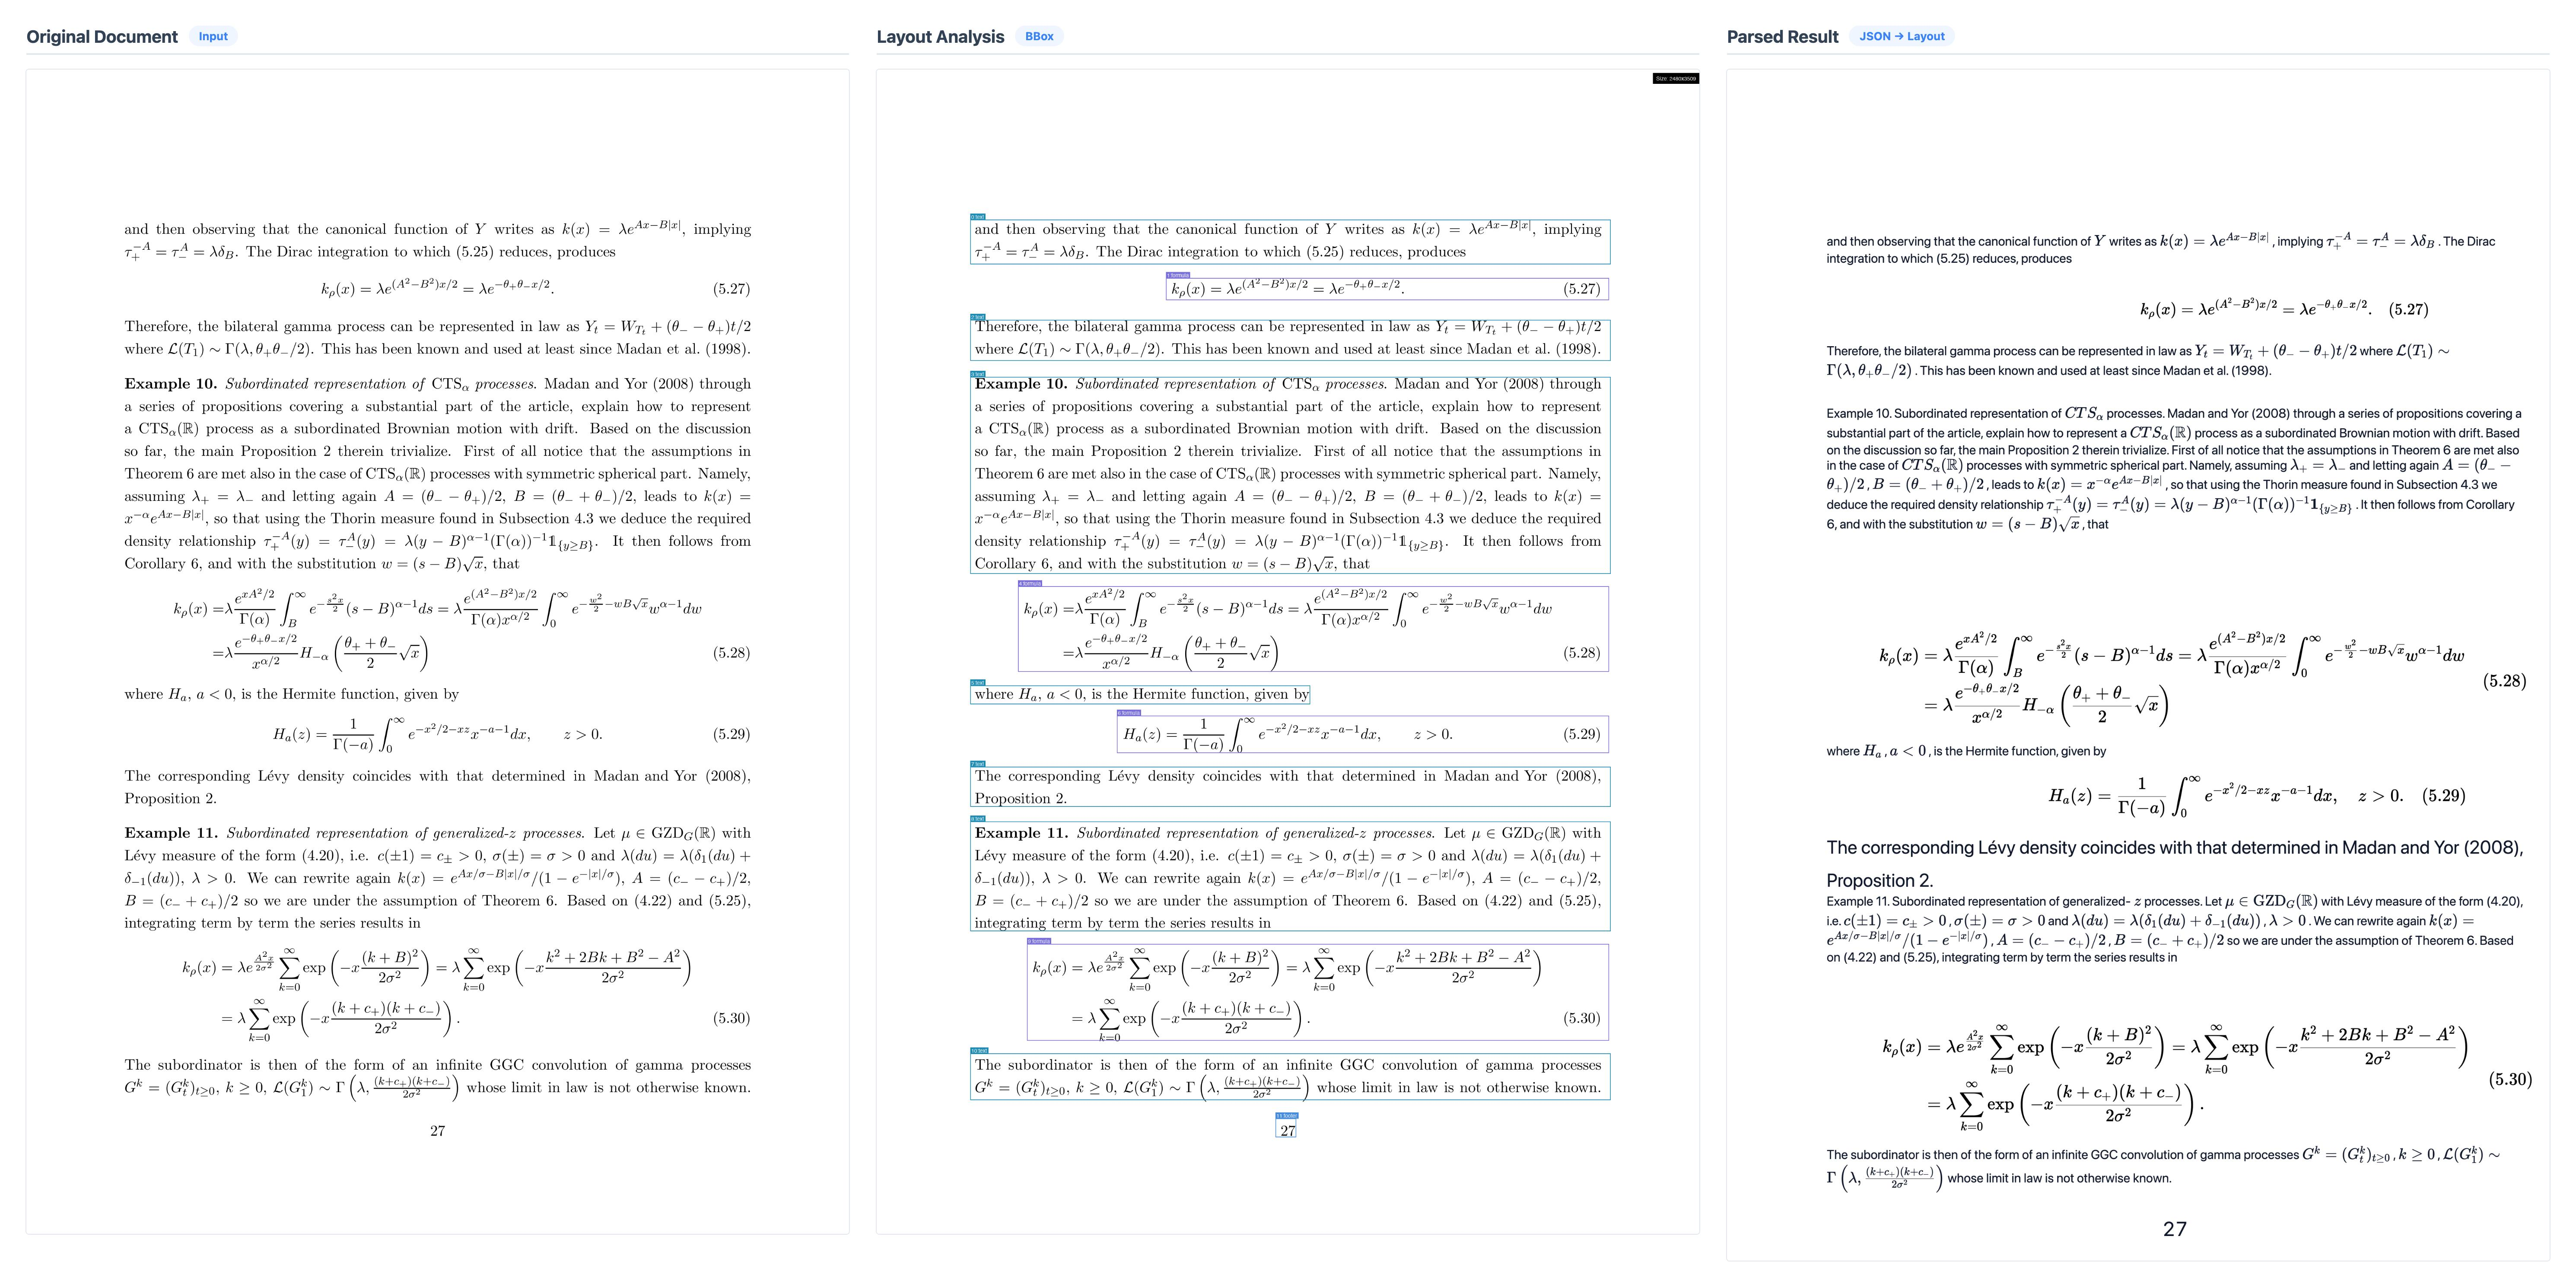
\includegraphics[width=\textwidth]{figures/visualization_results_arxiv.pdf}
    \caption{Visualization results of the arXiv paper image. The challenge is accurately preserving the structure of complex multi-line mathematical formulas, dense inline notations, and deeply nested subscripts/superscripts.}
    \label{fig:visualization_results_arxiv}
\end{figure*}

\begin{figure*}[htbp]
    \centering
    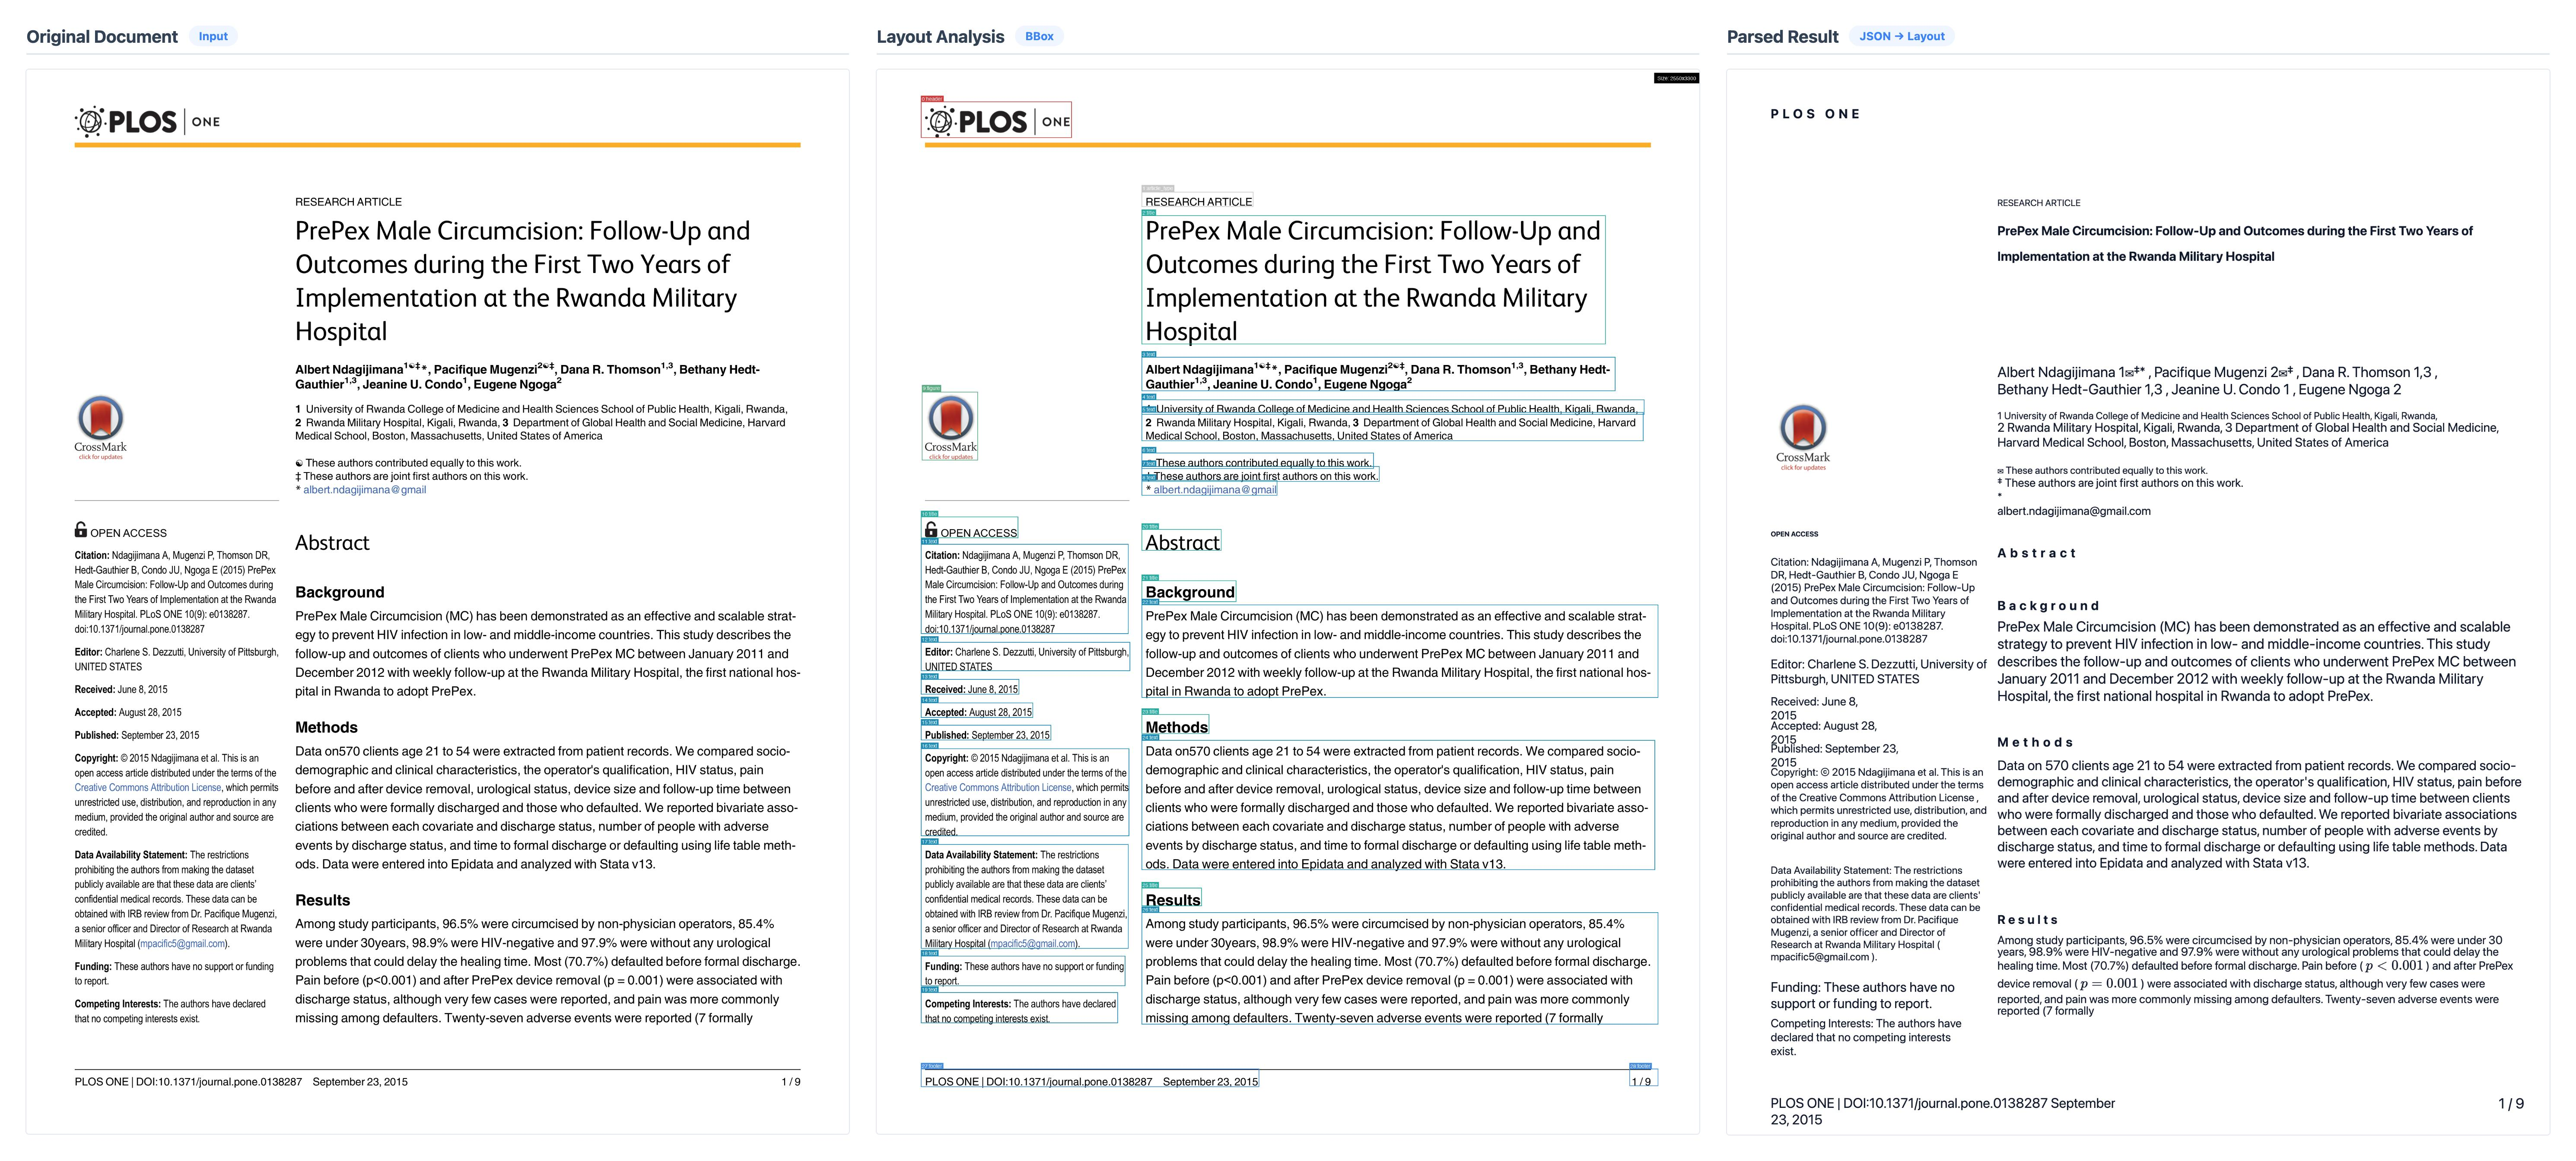
\includegraphics[width=\textwidth]{figures/visualization_results_magazine.pdf}
    \caption{Visualization results of the magazine image. The main difficulty is recovering the correct reading order within an asymmetric multi-column layout.}
    \label{fig:visualization_results_magazine}
\end{figure*}

\begin{figure*}[htbp]
    \centering
    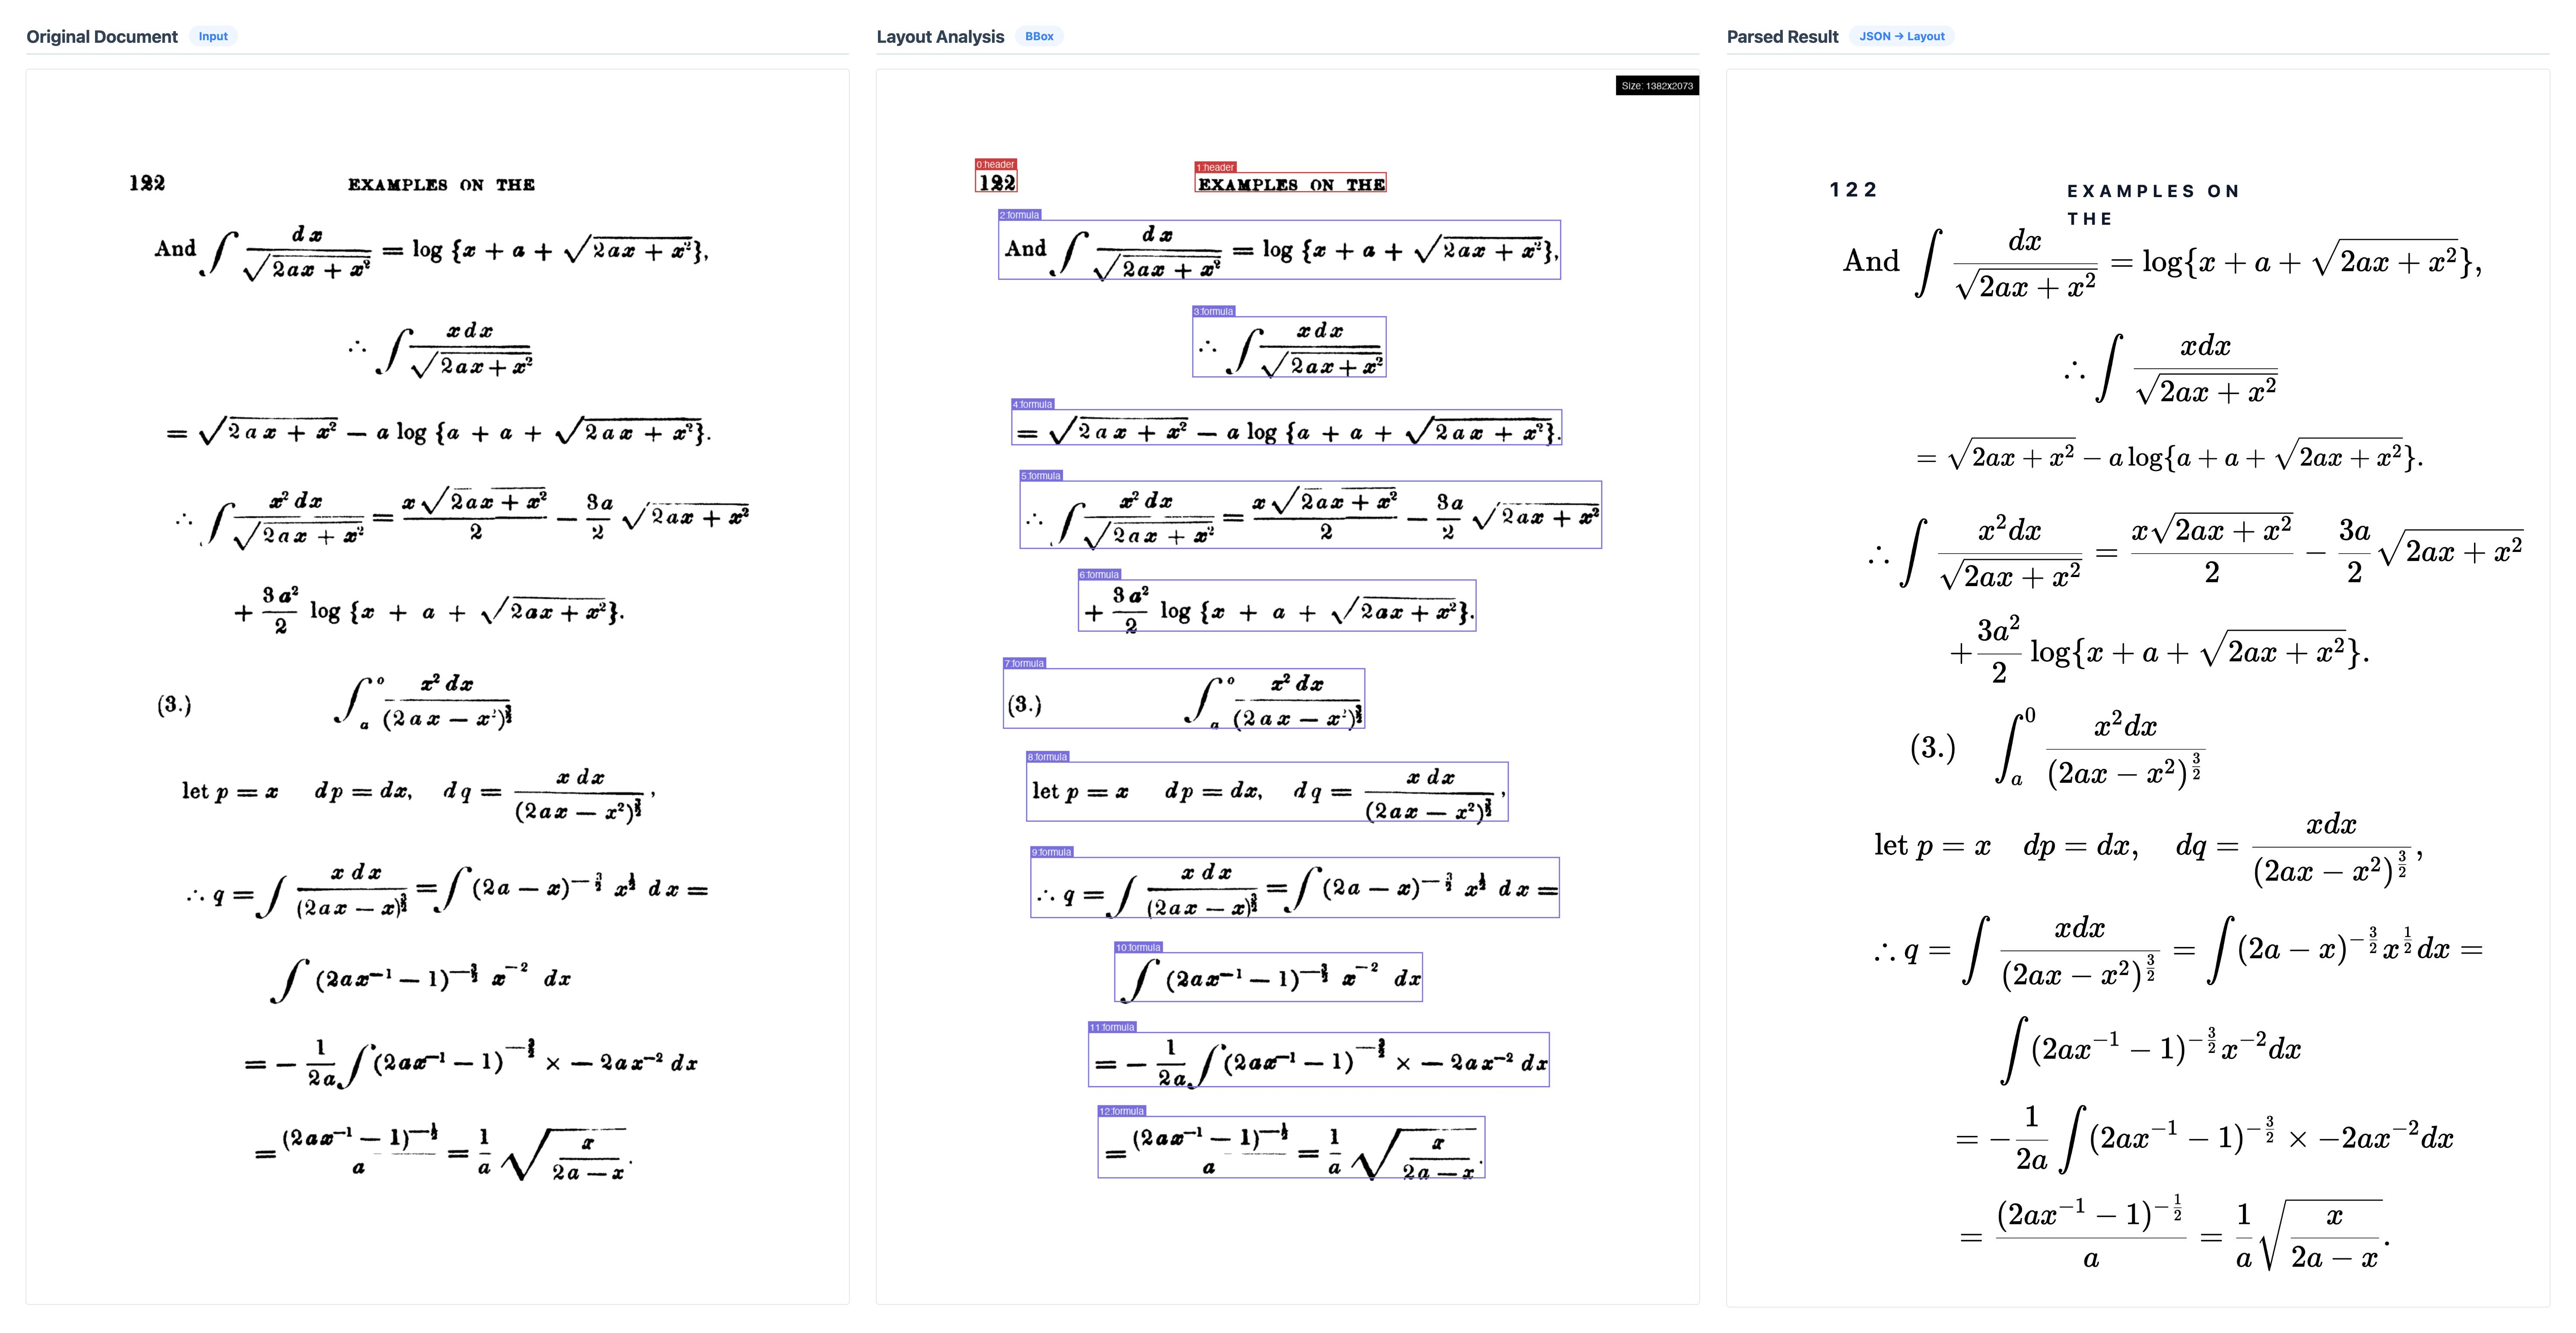
\includegraphics[width=\textwidth]{figures/visualization_results_old_scan_math.pdf}
    \caption{Visualization results of the old scanned math image. The challenge lies in recognizing text and symbols from severely degraded and blurred print.}
    \label{fig:visualization_results_old_scan_math}
\end{figure*}

\begin{figure*}[htbp]
    \centering
    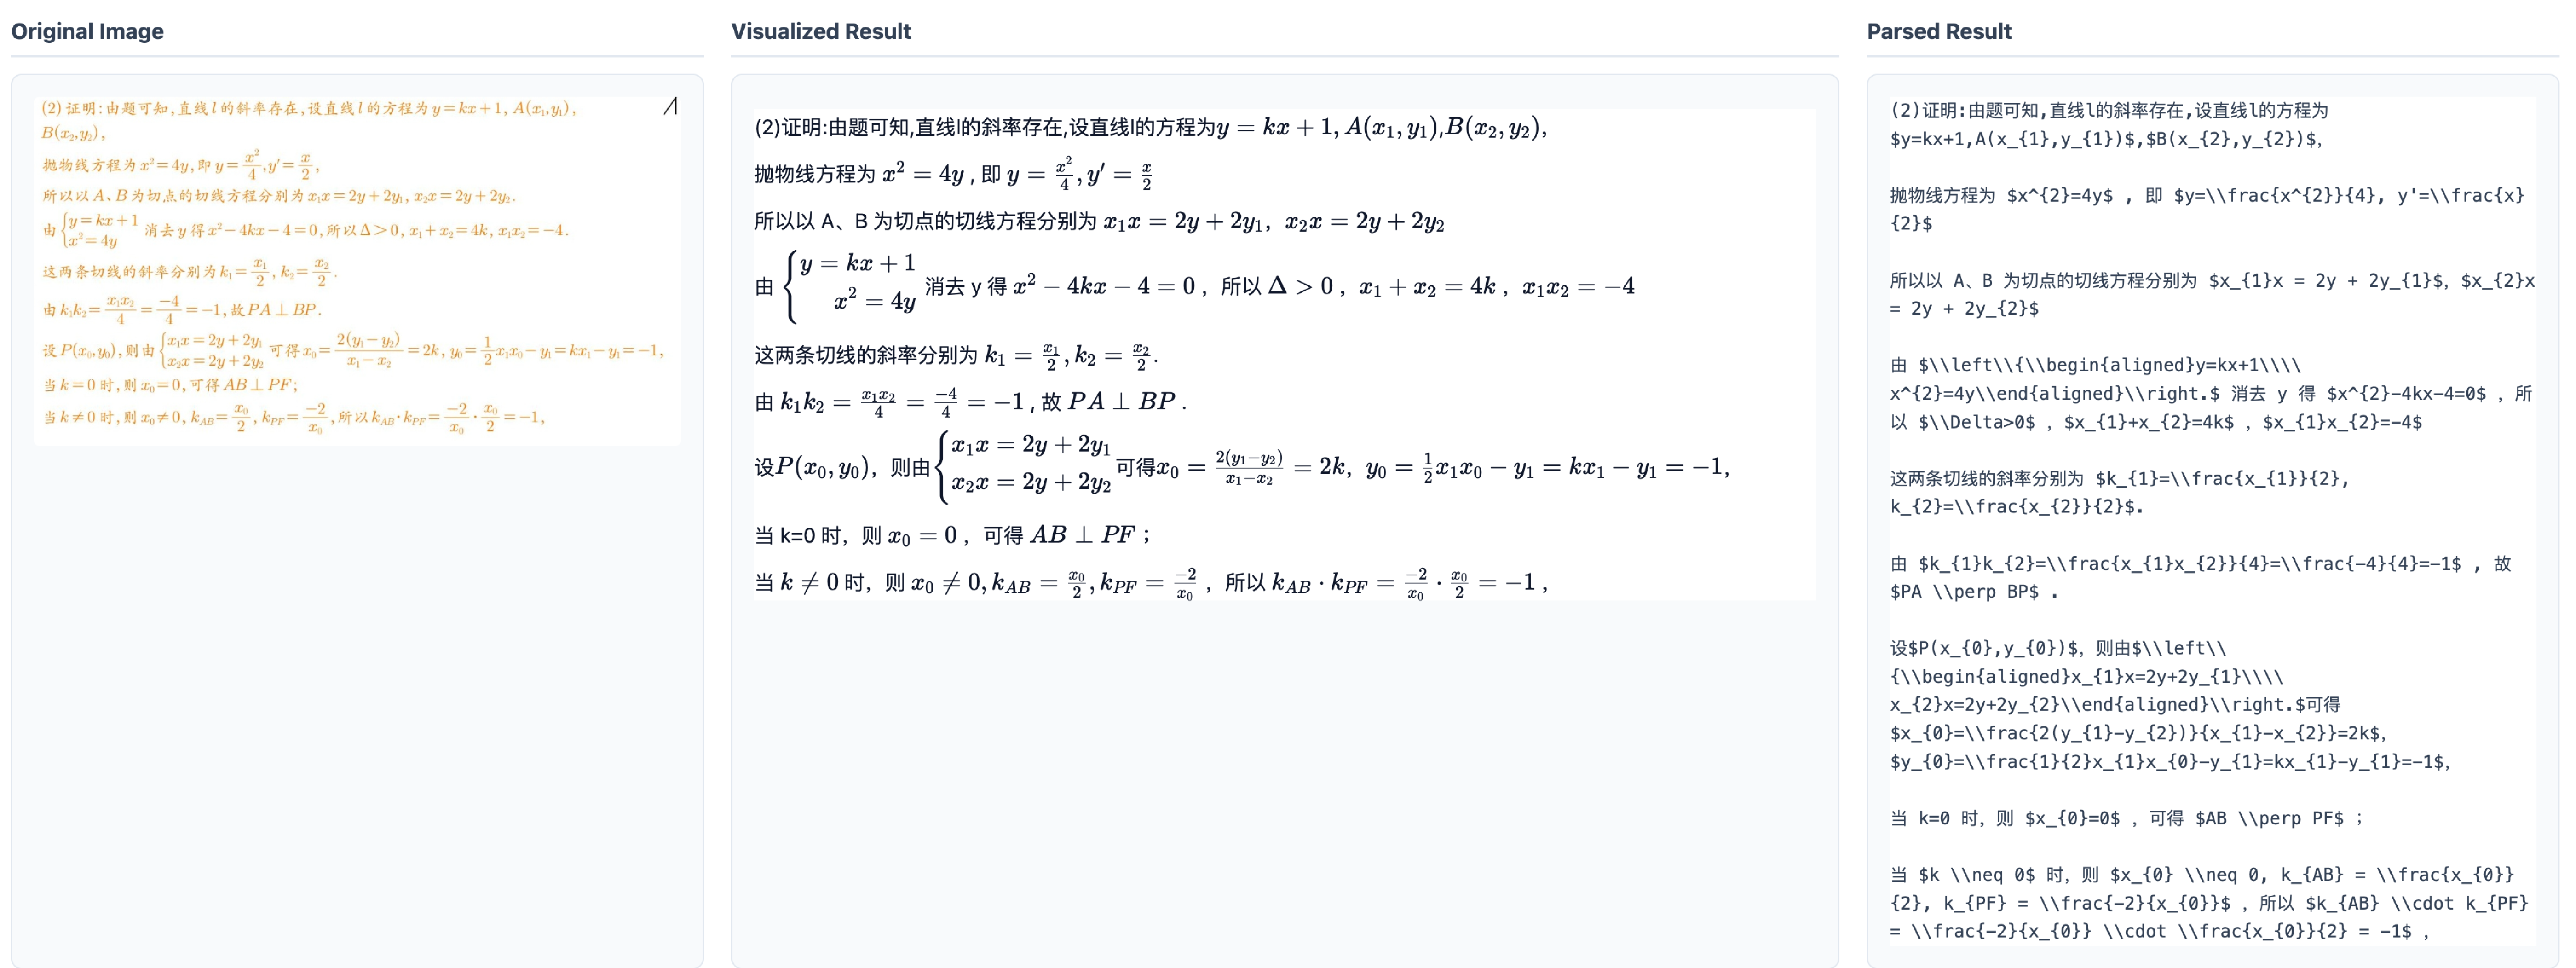
\includegraphics[width=\textwidth]{figures/visualization_results_text_parsing.pdf}
    \caption{Visualization results of the text parsing task. The challenge lies in faithfully transcribing densely written text interleaved with inline and displayed mathematical expressions while preserving the correct reading order across the full page.}
    \label{fig:visualization_results_text_parsing}
\end{figure*}

\begin{figure*}[htbp]
    \centering
    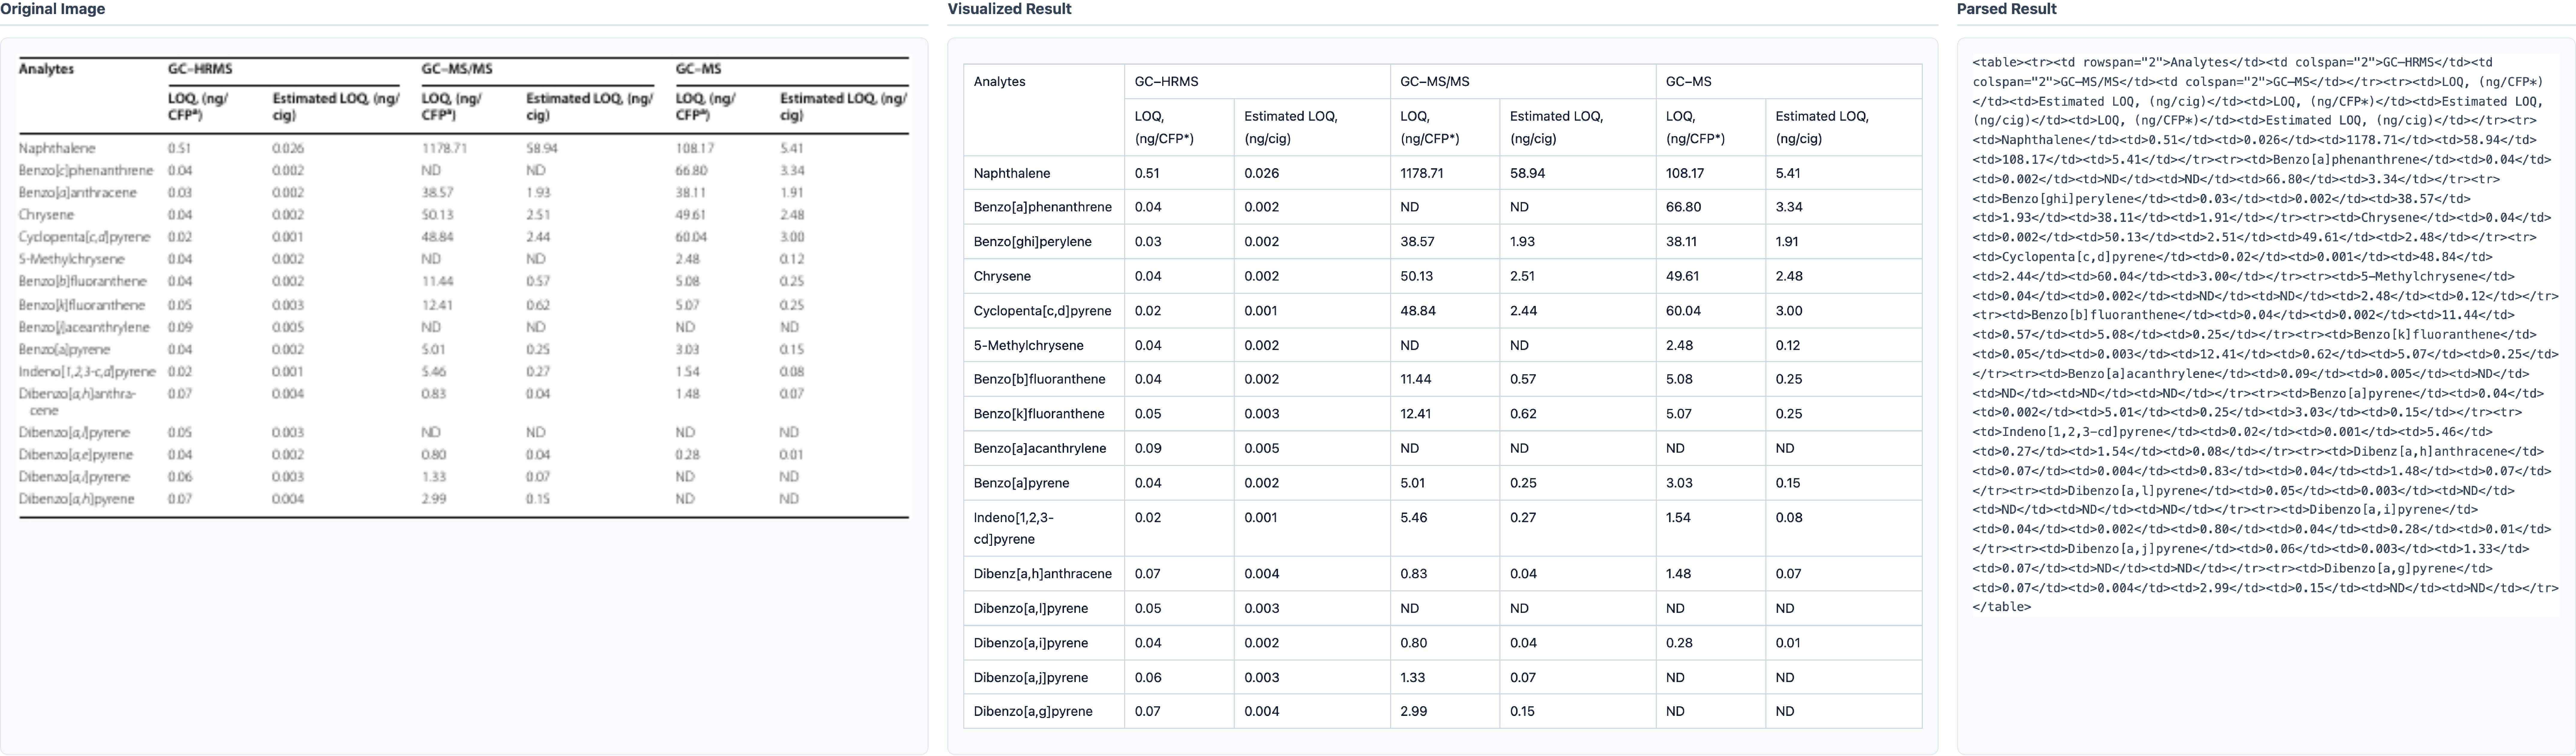
\includegraphics[width=\textwidth]{figures/visualization_results_table_parsing.pdf}
    \caption{Visualization results of the table parsing task. The difficulty involves reconstructing multi-level grouped column headers and aligning numerous numeric cells precisely within a dense scientific table.}
    \label{fig:visualization_results_table_parsing}
\end{figure*}

\begin{figure*}[htbp]
    \centering
    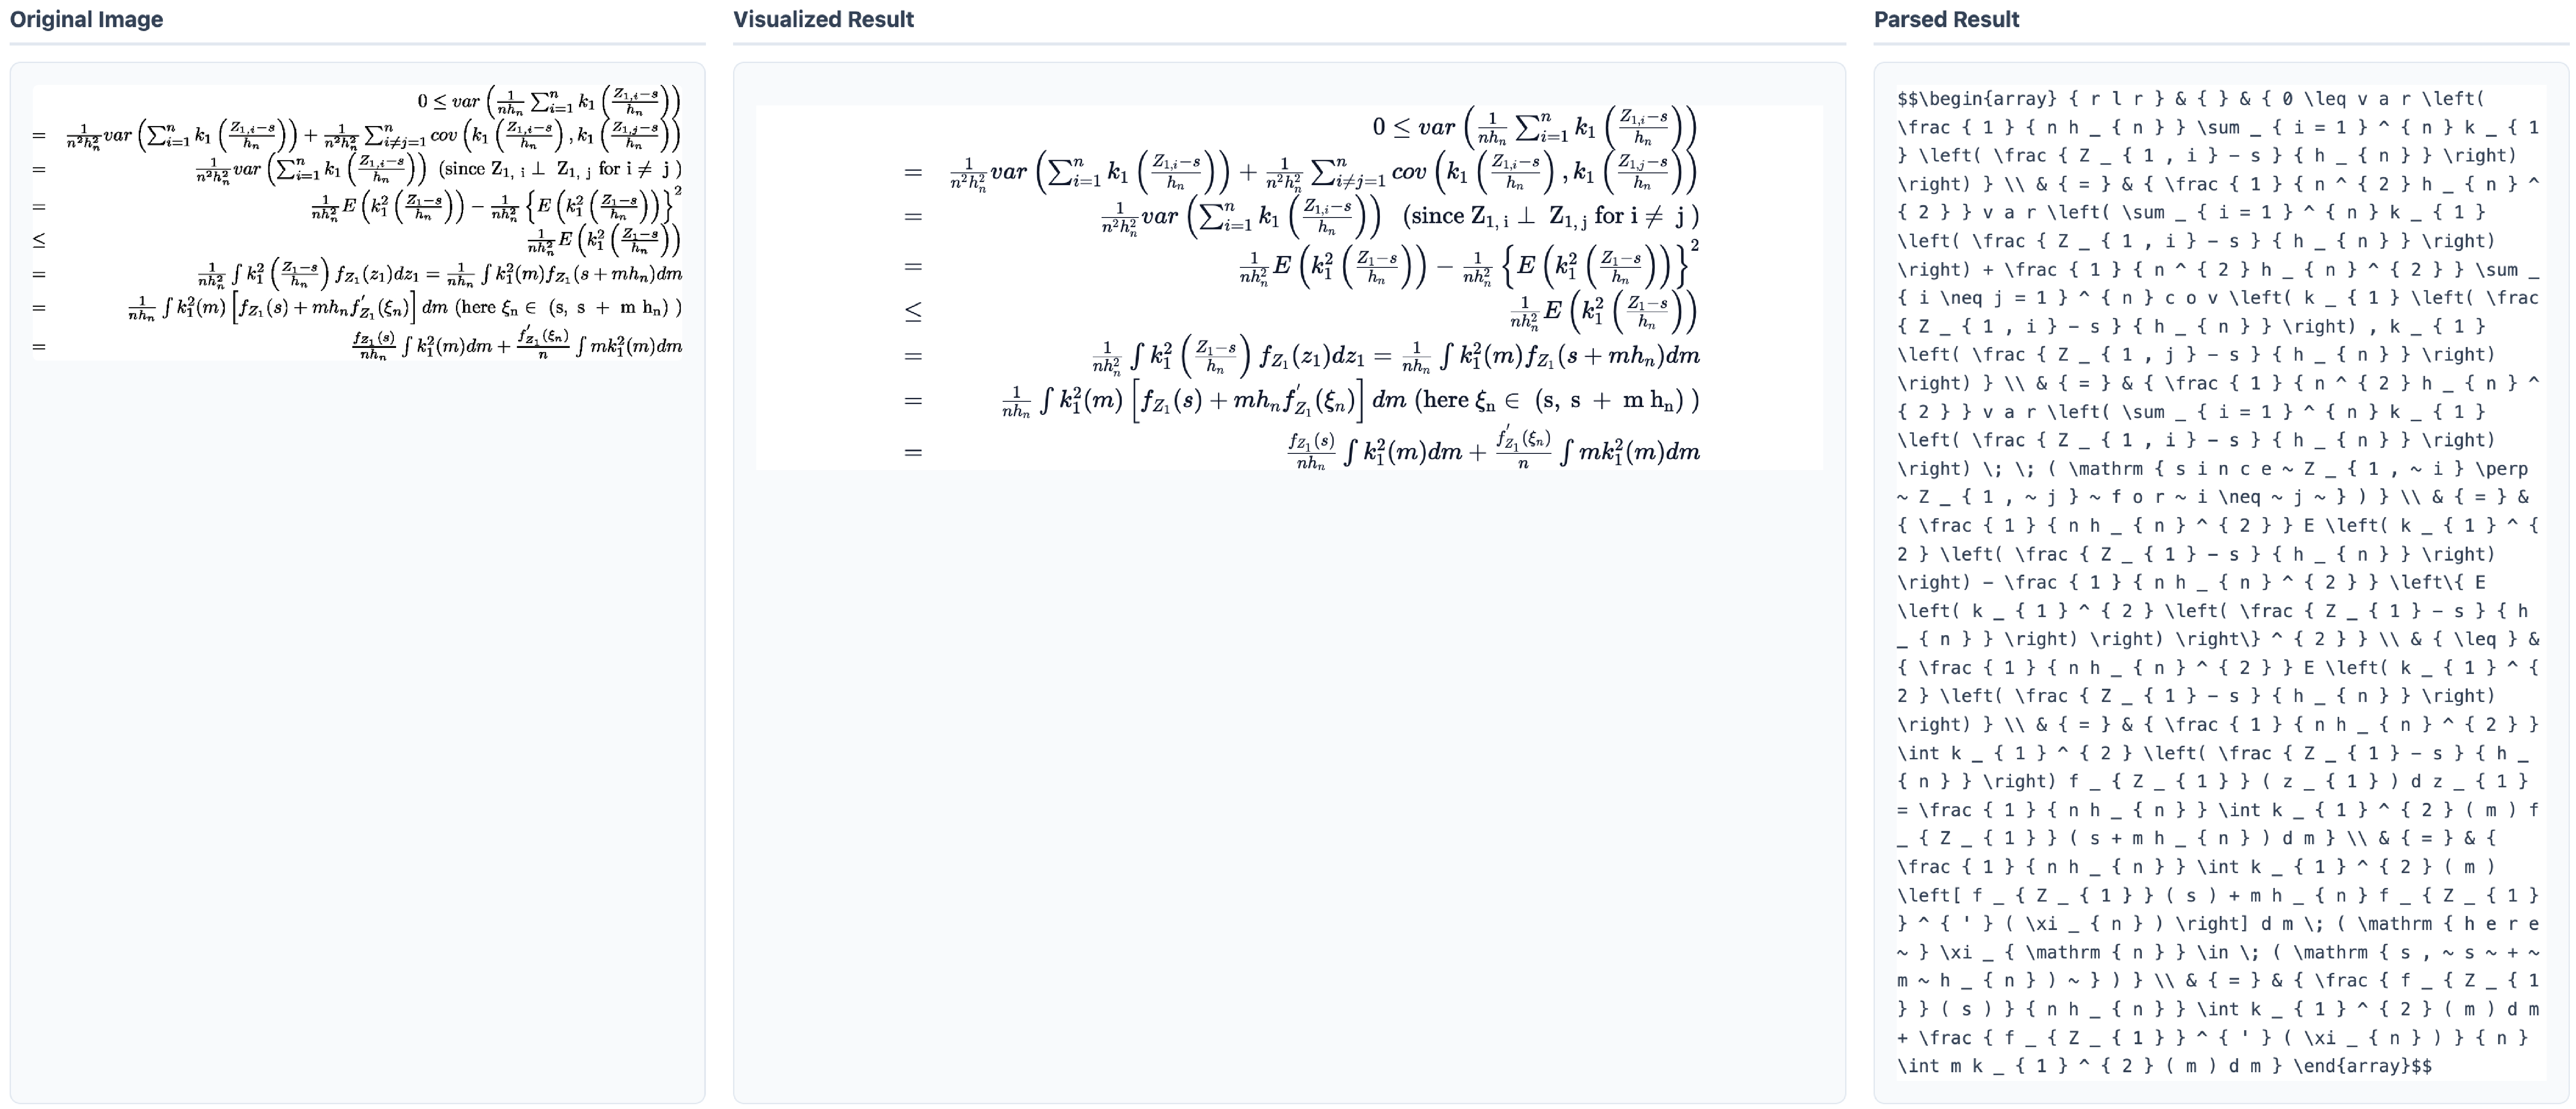
\includegraphics[width=\textwidth]{figures/visualization_results_formula_parsing.pdf}
    \caption{Visualization results of the formula parsing task. The challenge is accurately transcribing a multi-line derivation with nested fractions, summation and expectation operators, integrals, and densely stacked subscripts and superscripts into valid LaTeX.}
    \label{fig:visualization_results_formula_parsing}
\end{figure*}

\begin{figure*}[htbp]
    \centering
    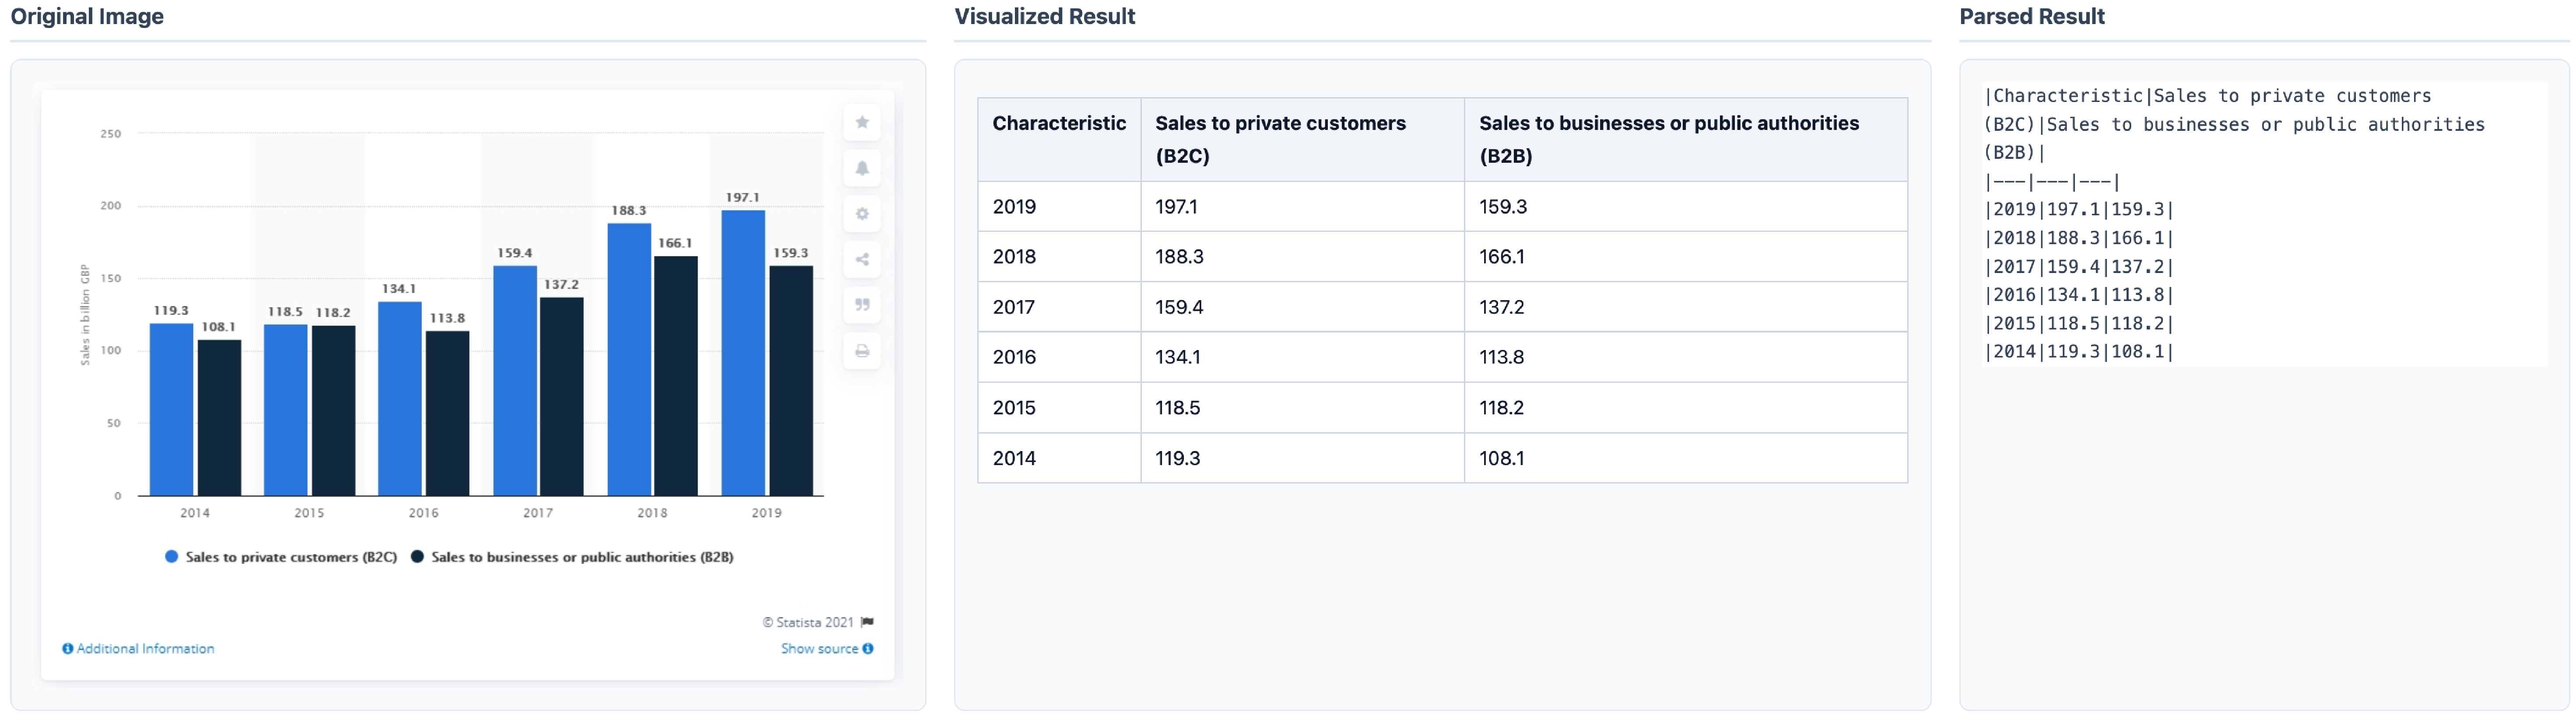
\includegraphics[width=\textwidth]{figures/visualization_results_chart2table.pdf}
    \caption{Visualization results of the Chart-to-Table task. The difficulty lies in reading the numeric value of each grouped bar and associating it with the correct category and data series to recover a structured table.}
    \label{fig:visualization_results_chart2table}
\end{figure*}

\begin{figure*}[htbp]
    \centering
    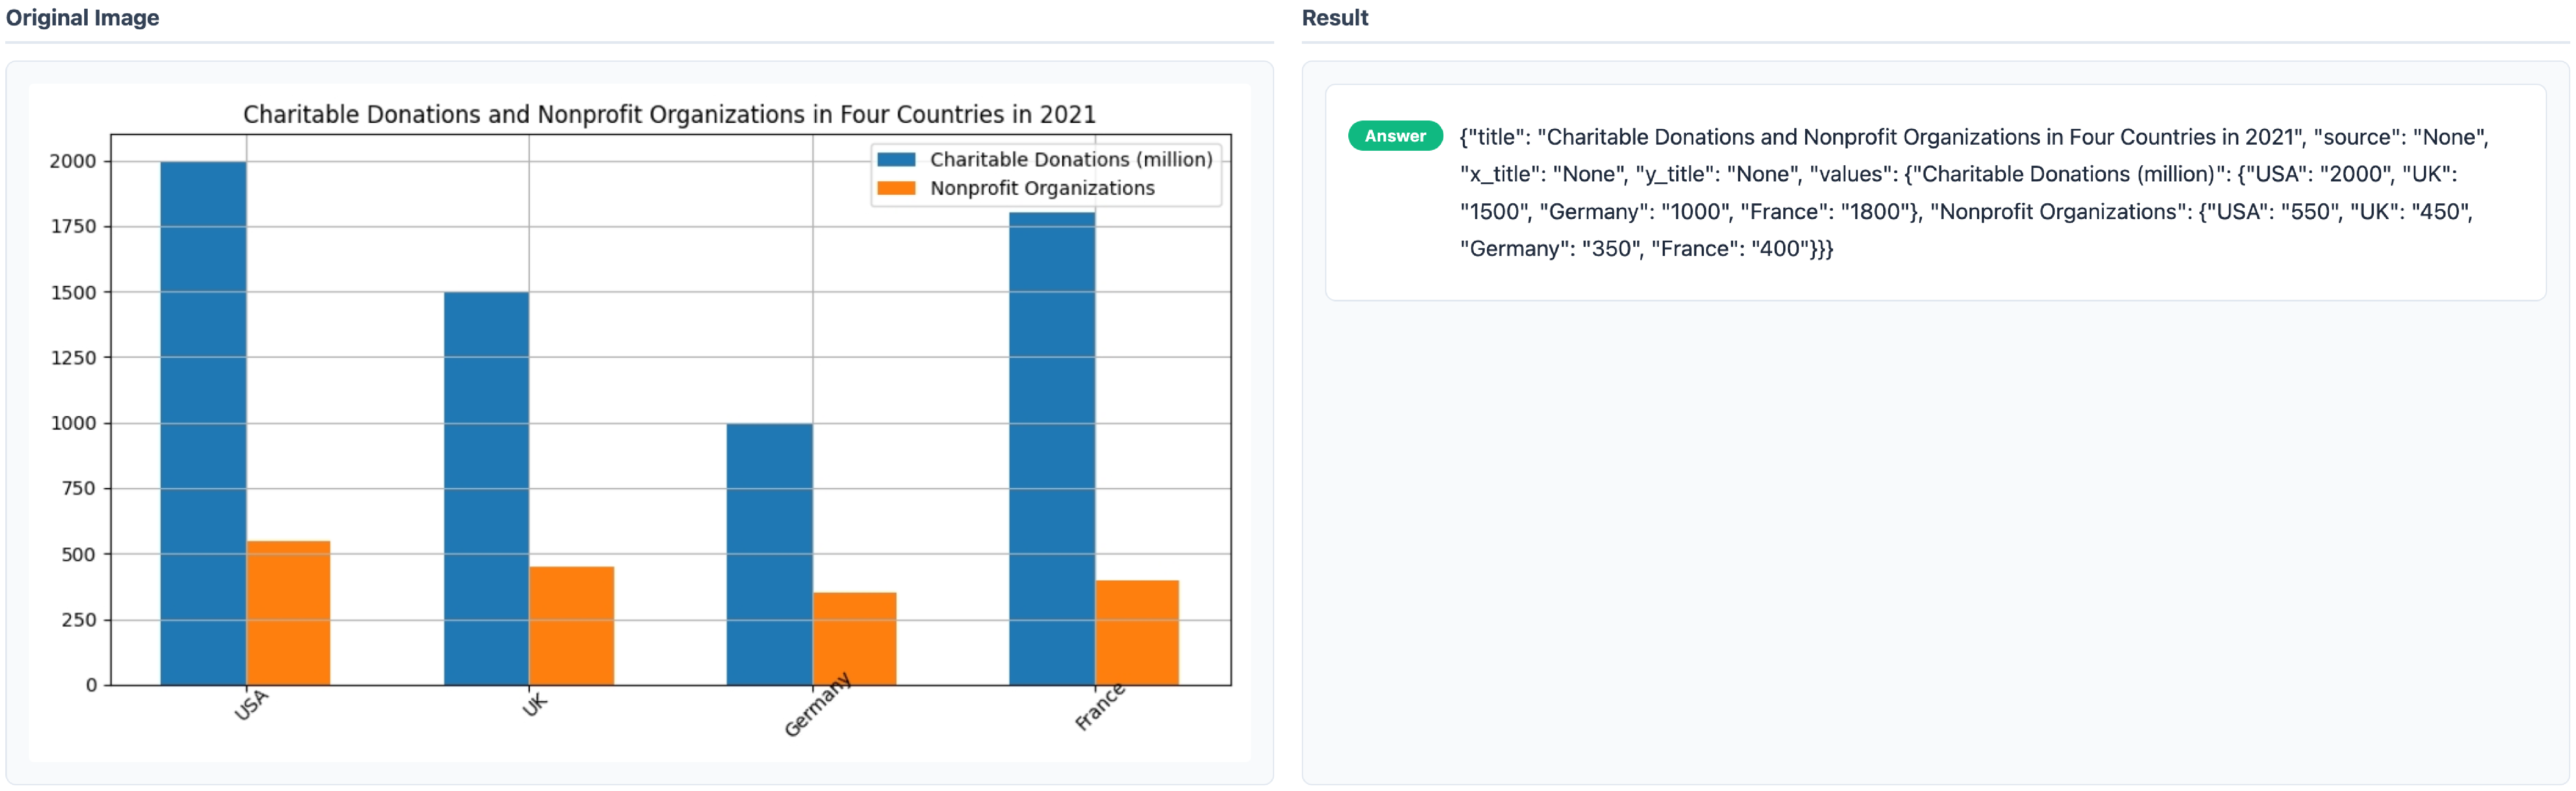
\includegraphics[width=\textwidth]{figures/visualization_results_chart2json.pdf}
    \caption{Visualization results of the Chart-to-JSON task. The challenge is extracting the title, axis labels, and hierarchically grouped data values into a well-formed, schema-consistent JSON representation.}
    \label{fig:visualization_results_chart2json}
\end{figure*}

\begin{figure*}[htbp]
    \centering
    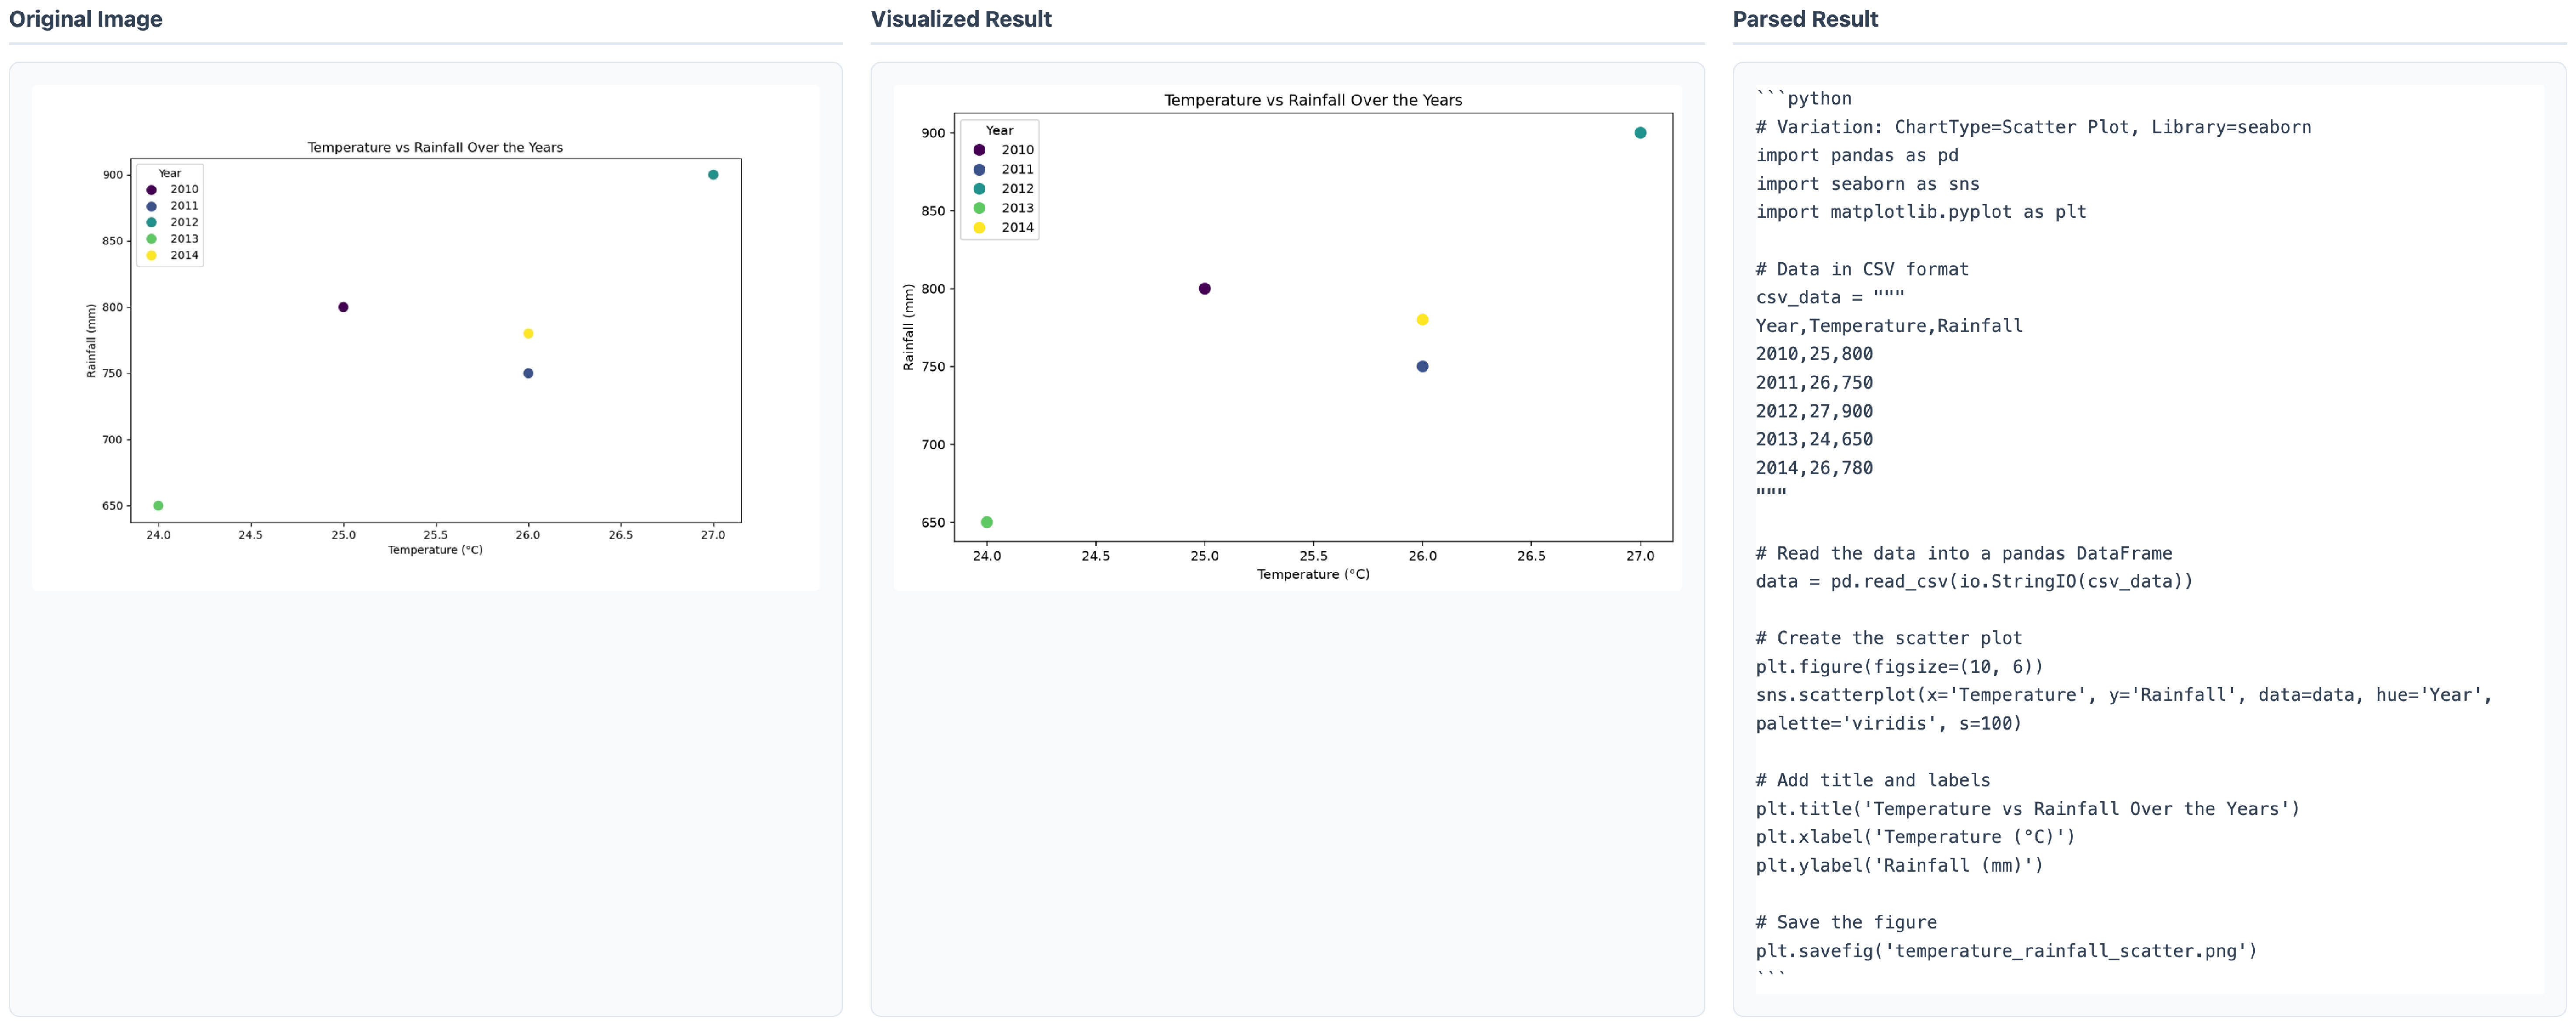
\includegraphics[width=\textwidth]{figures/visualization_results_chart2code.pdf}
    \caption{Visualization results of the Chart-to-Code task. The difficulty involves inferring the chart type, underlying data, and visual styling to generate executable plotting code that faithfully reproduces the original figure.}
    \label{fig:visualization_results_chart2code}
\end{figure*}

\begin{figure*}[htbp]
    \centering
    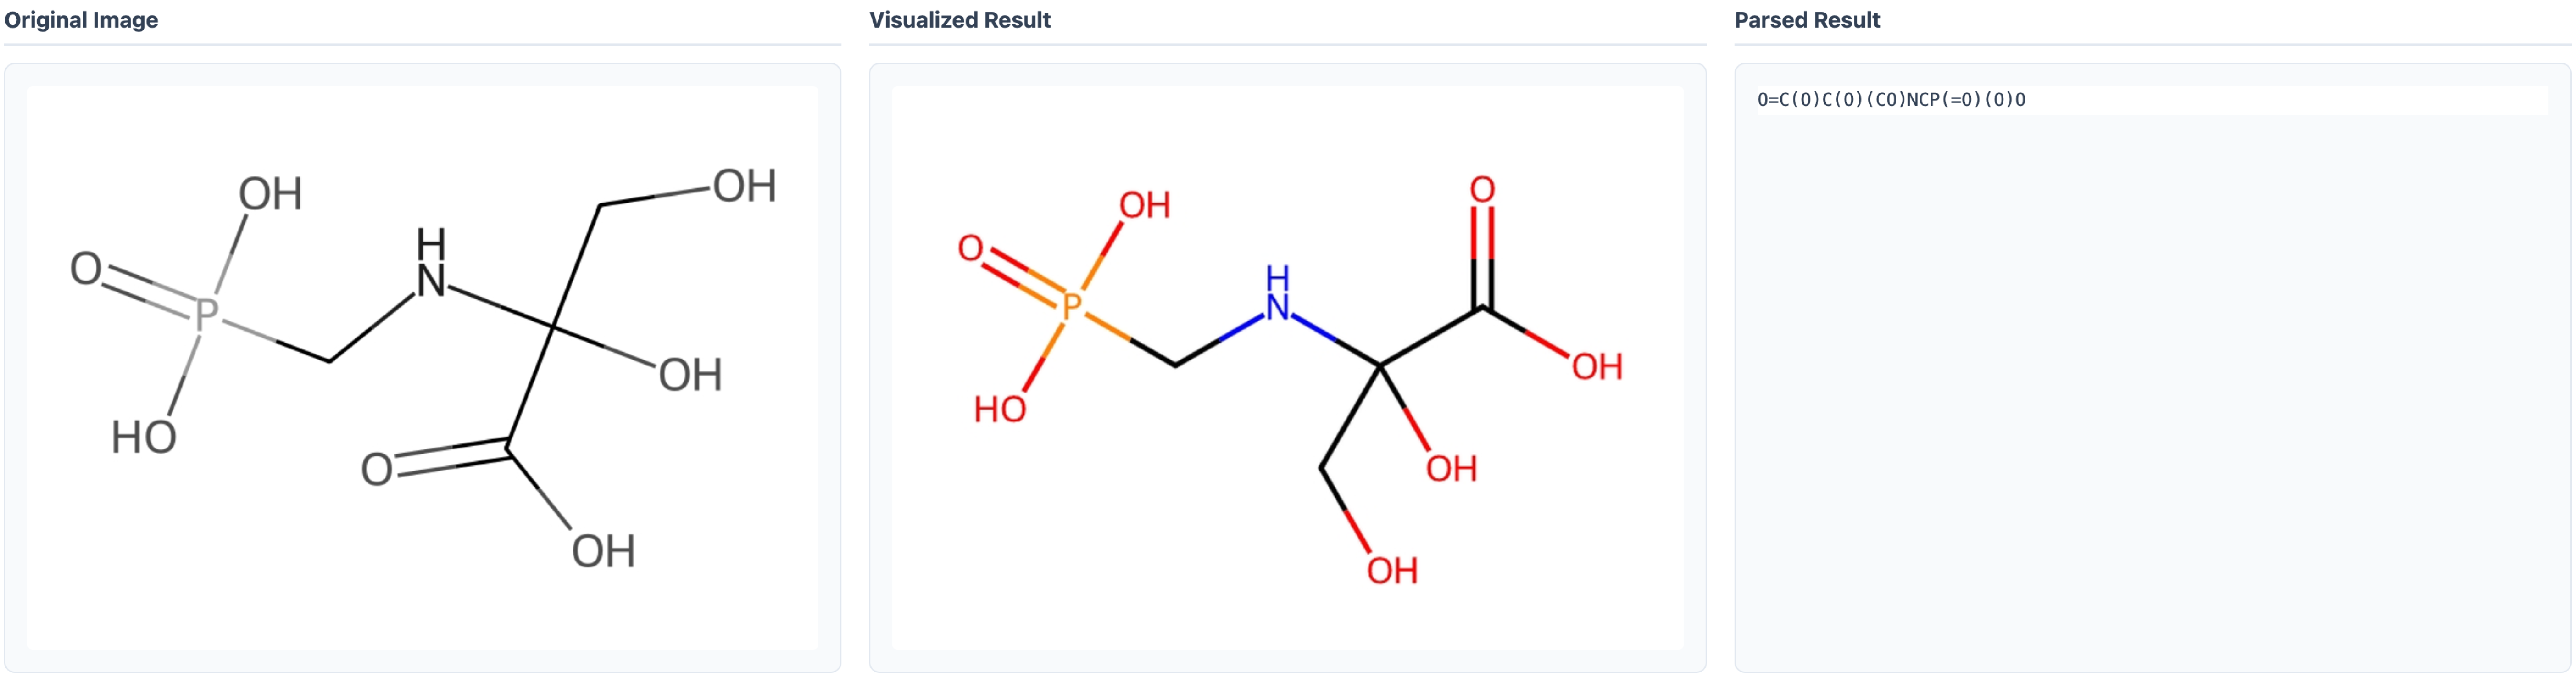
\includegraphics[width=\textwidth]{figures/visualization_results_chem2smiles.pdf}
    \caption{Visualization results of the Chemical-to-SMILES task. The challenge is recognizing atoms, bonds, and functional groups in the molecular diagram and converting the two-dimensional structure into a valid linear SMILES string.}
    \label{fig:visualization_results_chem2smiles}
\end{figure*}

\begin{figure*}[htbp]
    \centering
    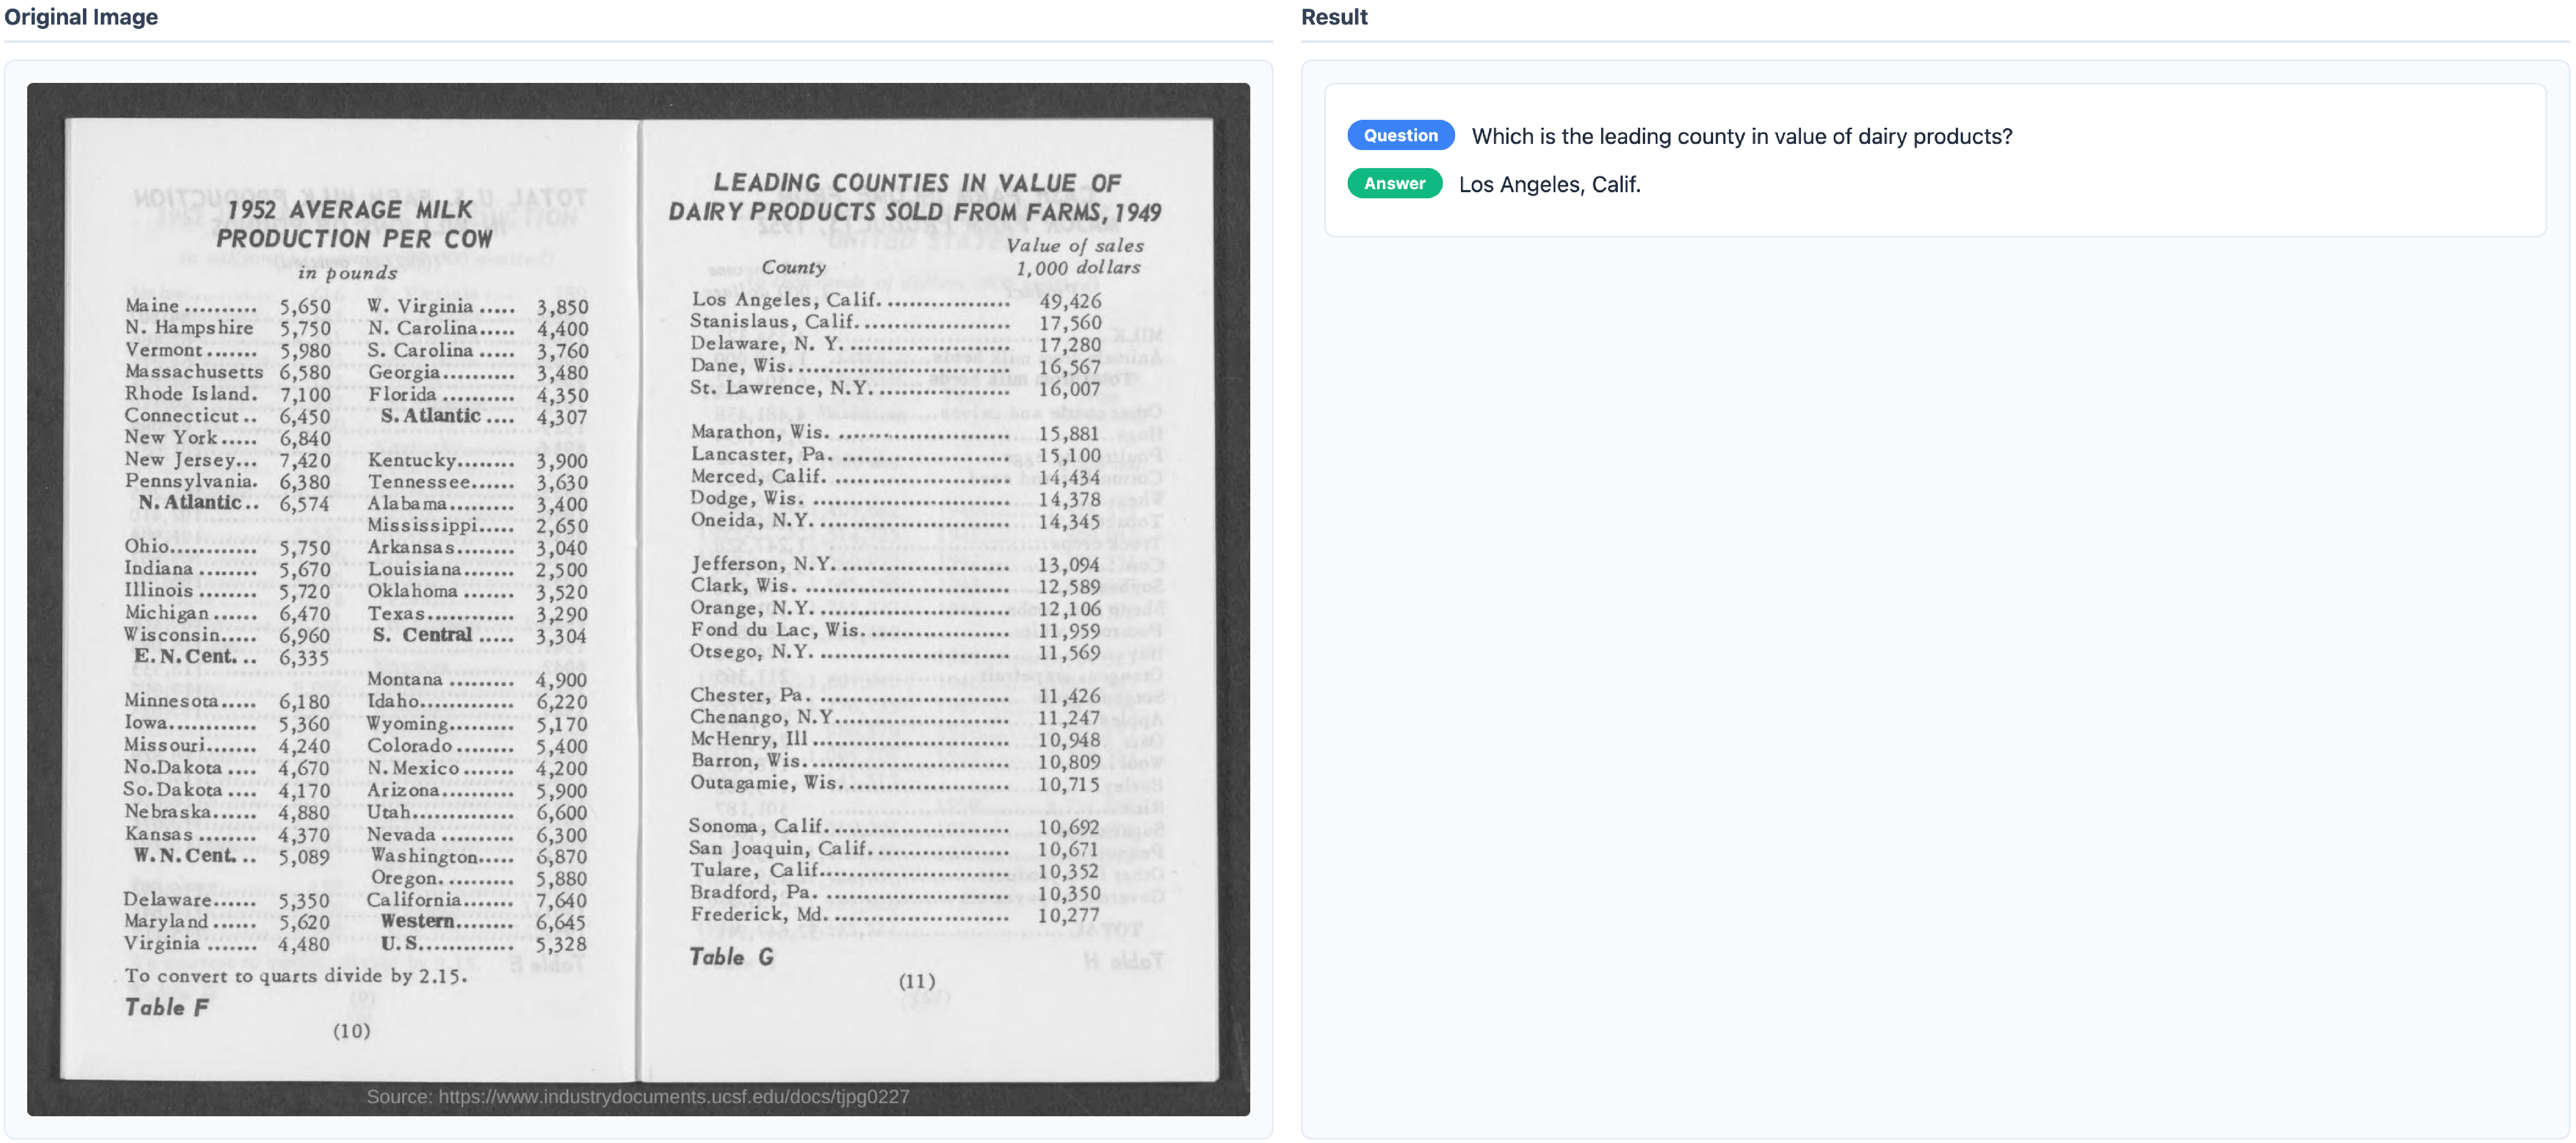
\includegraphics[width=\textwidth]{figures/visualization_results_docvqa.pdf}
    \caption{Visualization results of the DocVQA task. The challenge lies in locating the relevant table within a dense multi-table document page and reading the top-ranked entry to answer the question.}
    \label{fig:visualization_results_docvqa}
\end{figure*}

\begin{figure*}[htbp]
    \centering
    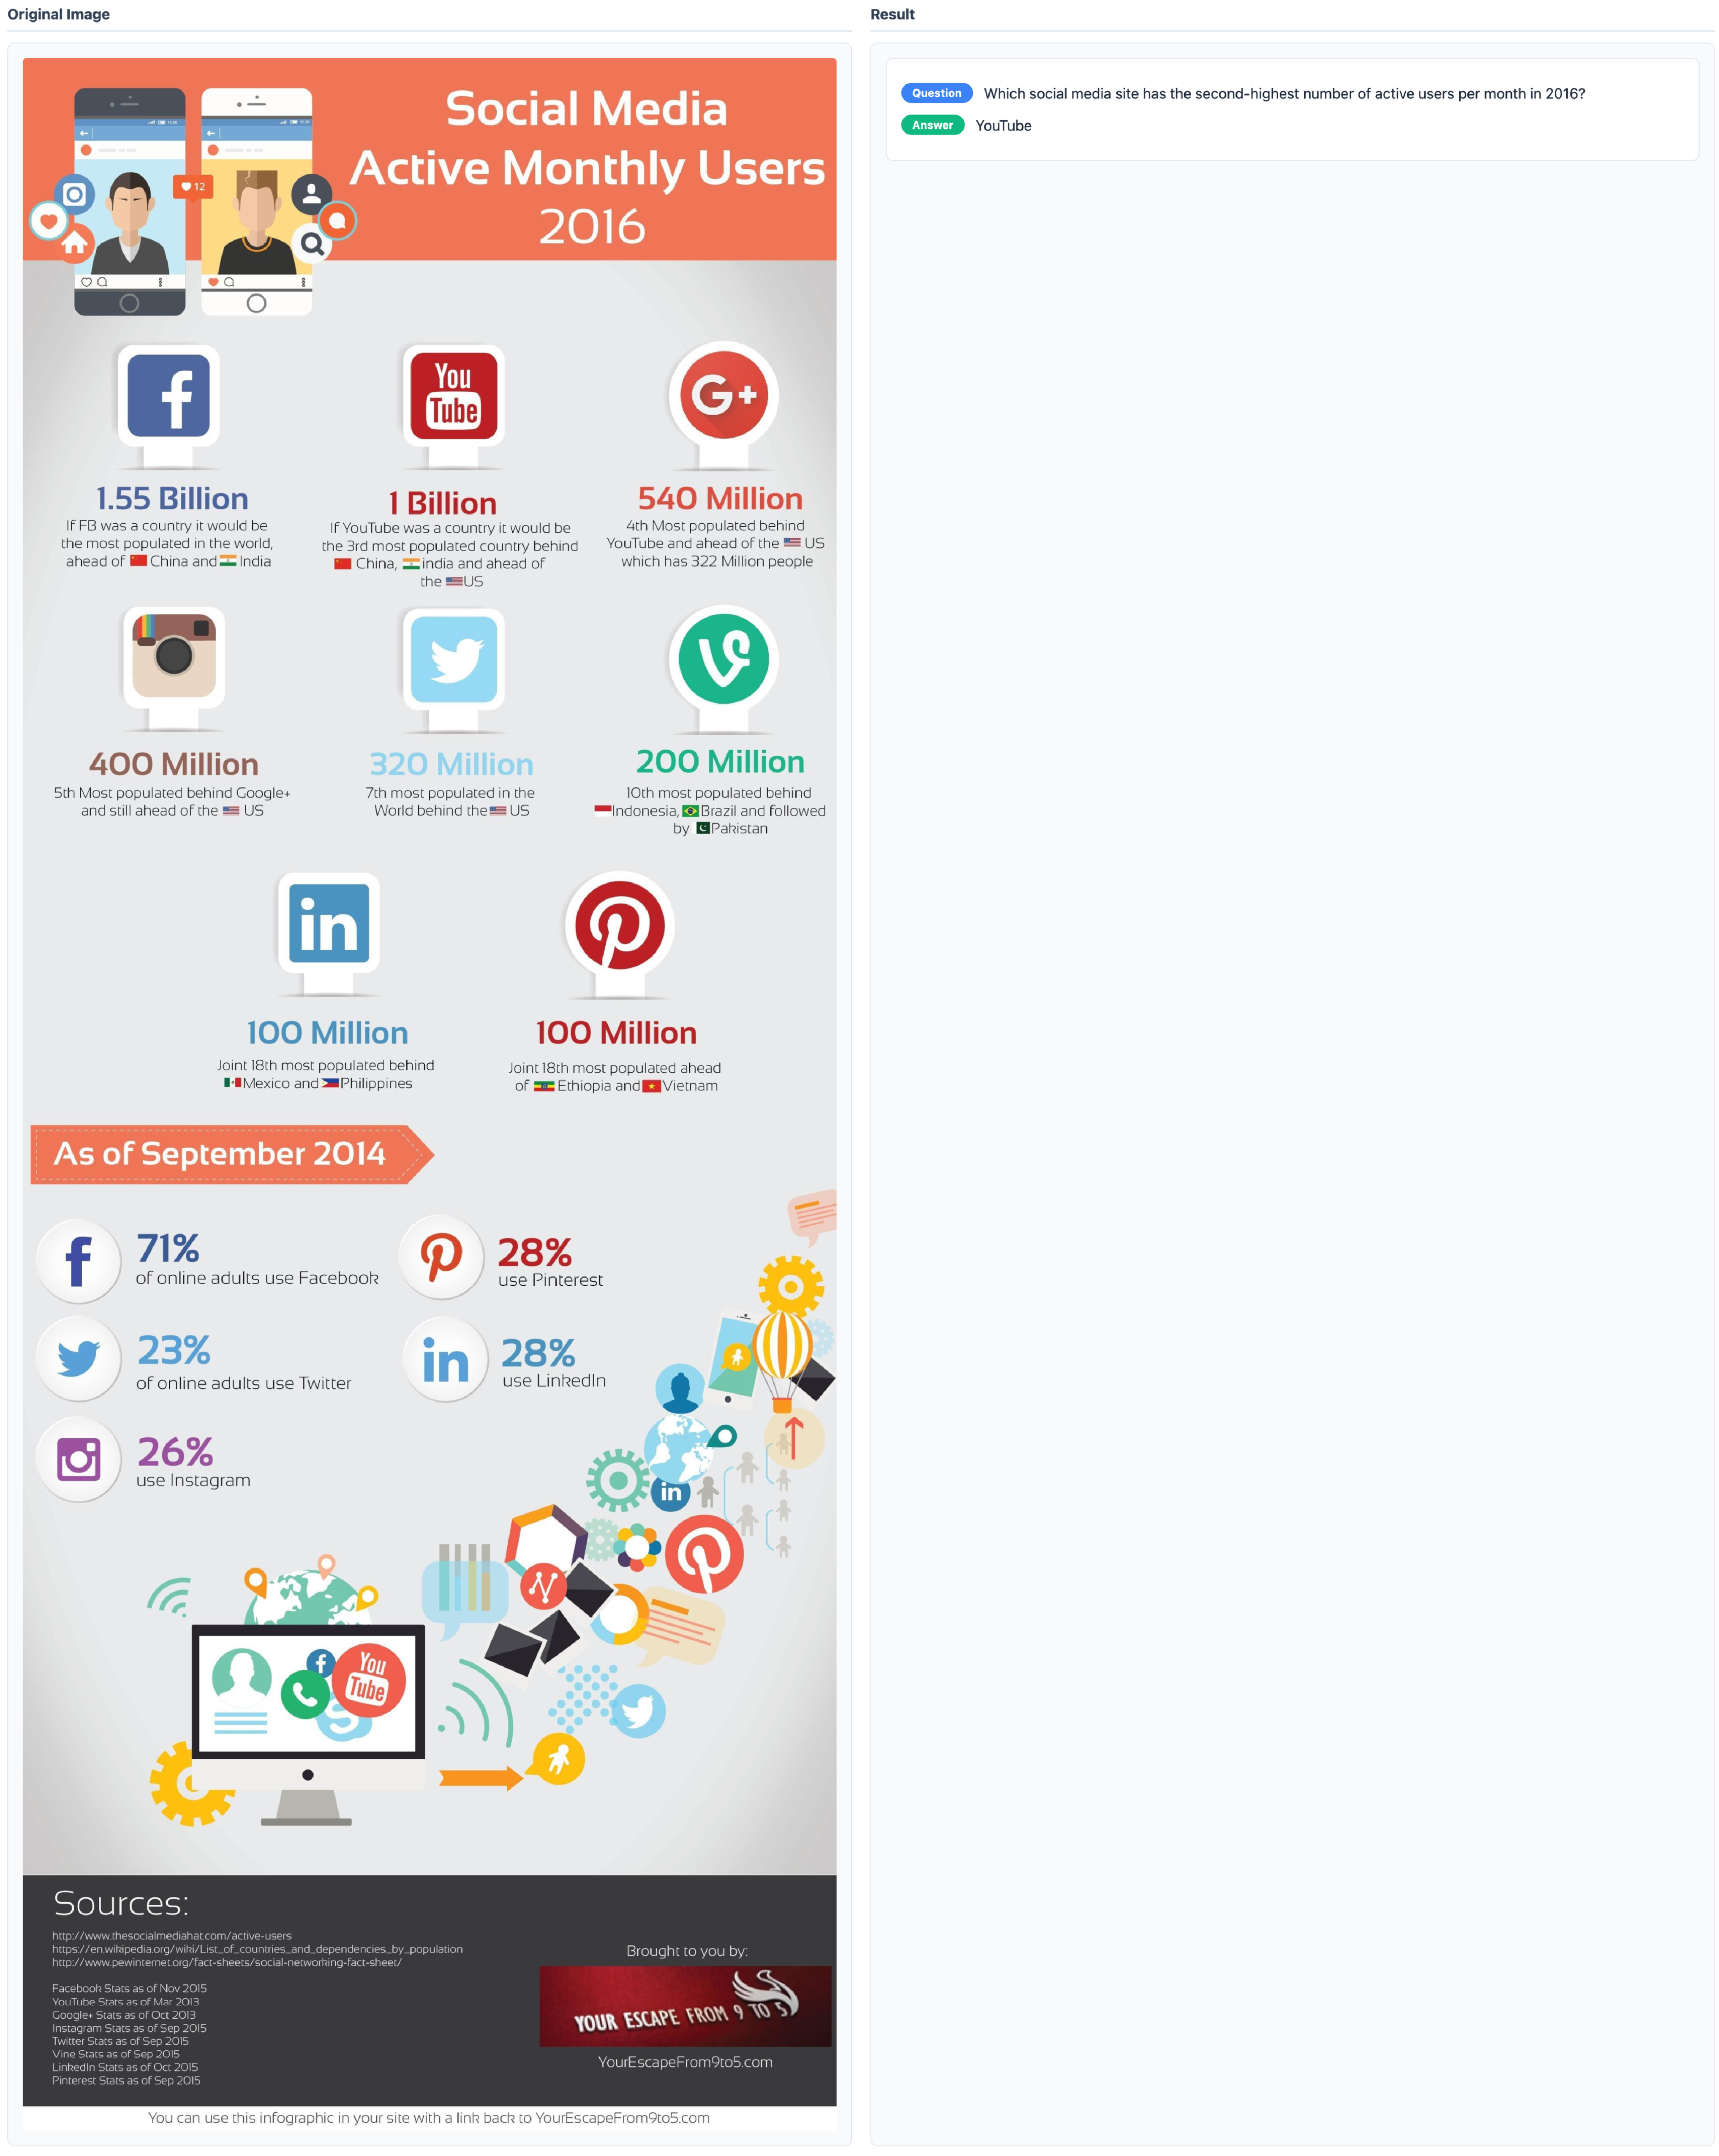
\includegraphics[width=\textwidth]{figures/visualization_results_infovqa.pdf}
    \caption{Visualization results of the InfoVQA task. The difficulty lies in reasoning over a visually complex infographic with scattered icons, stylized numbers, and a non-linear layout to compare and rank quantities.}
    \label{fig:visualization_results_infovqa}
\end{figure*}

\begin{figure*}[htbp]
    \centering
    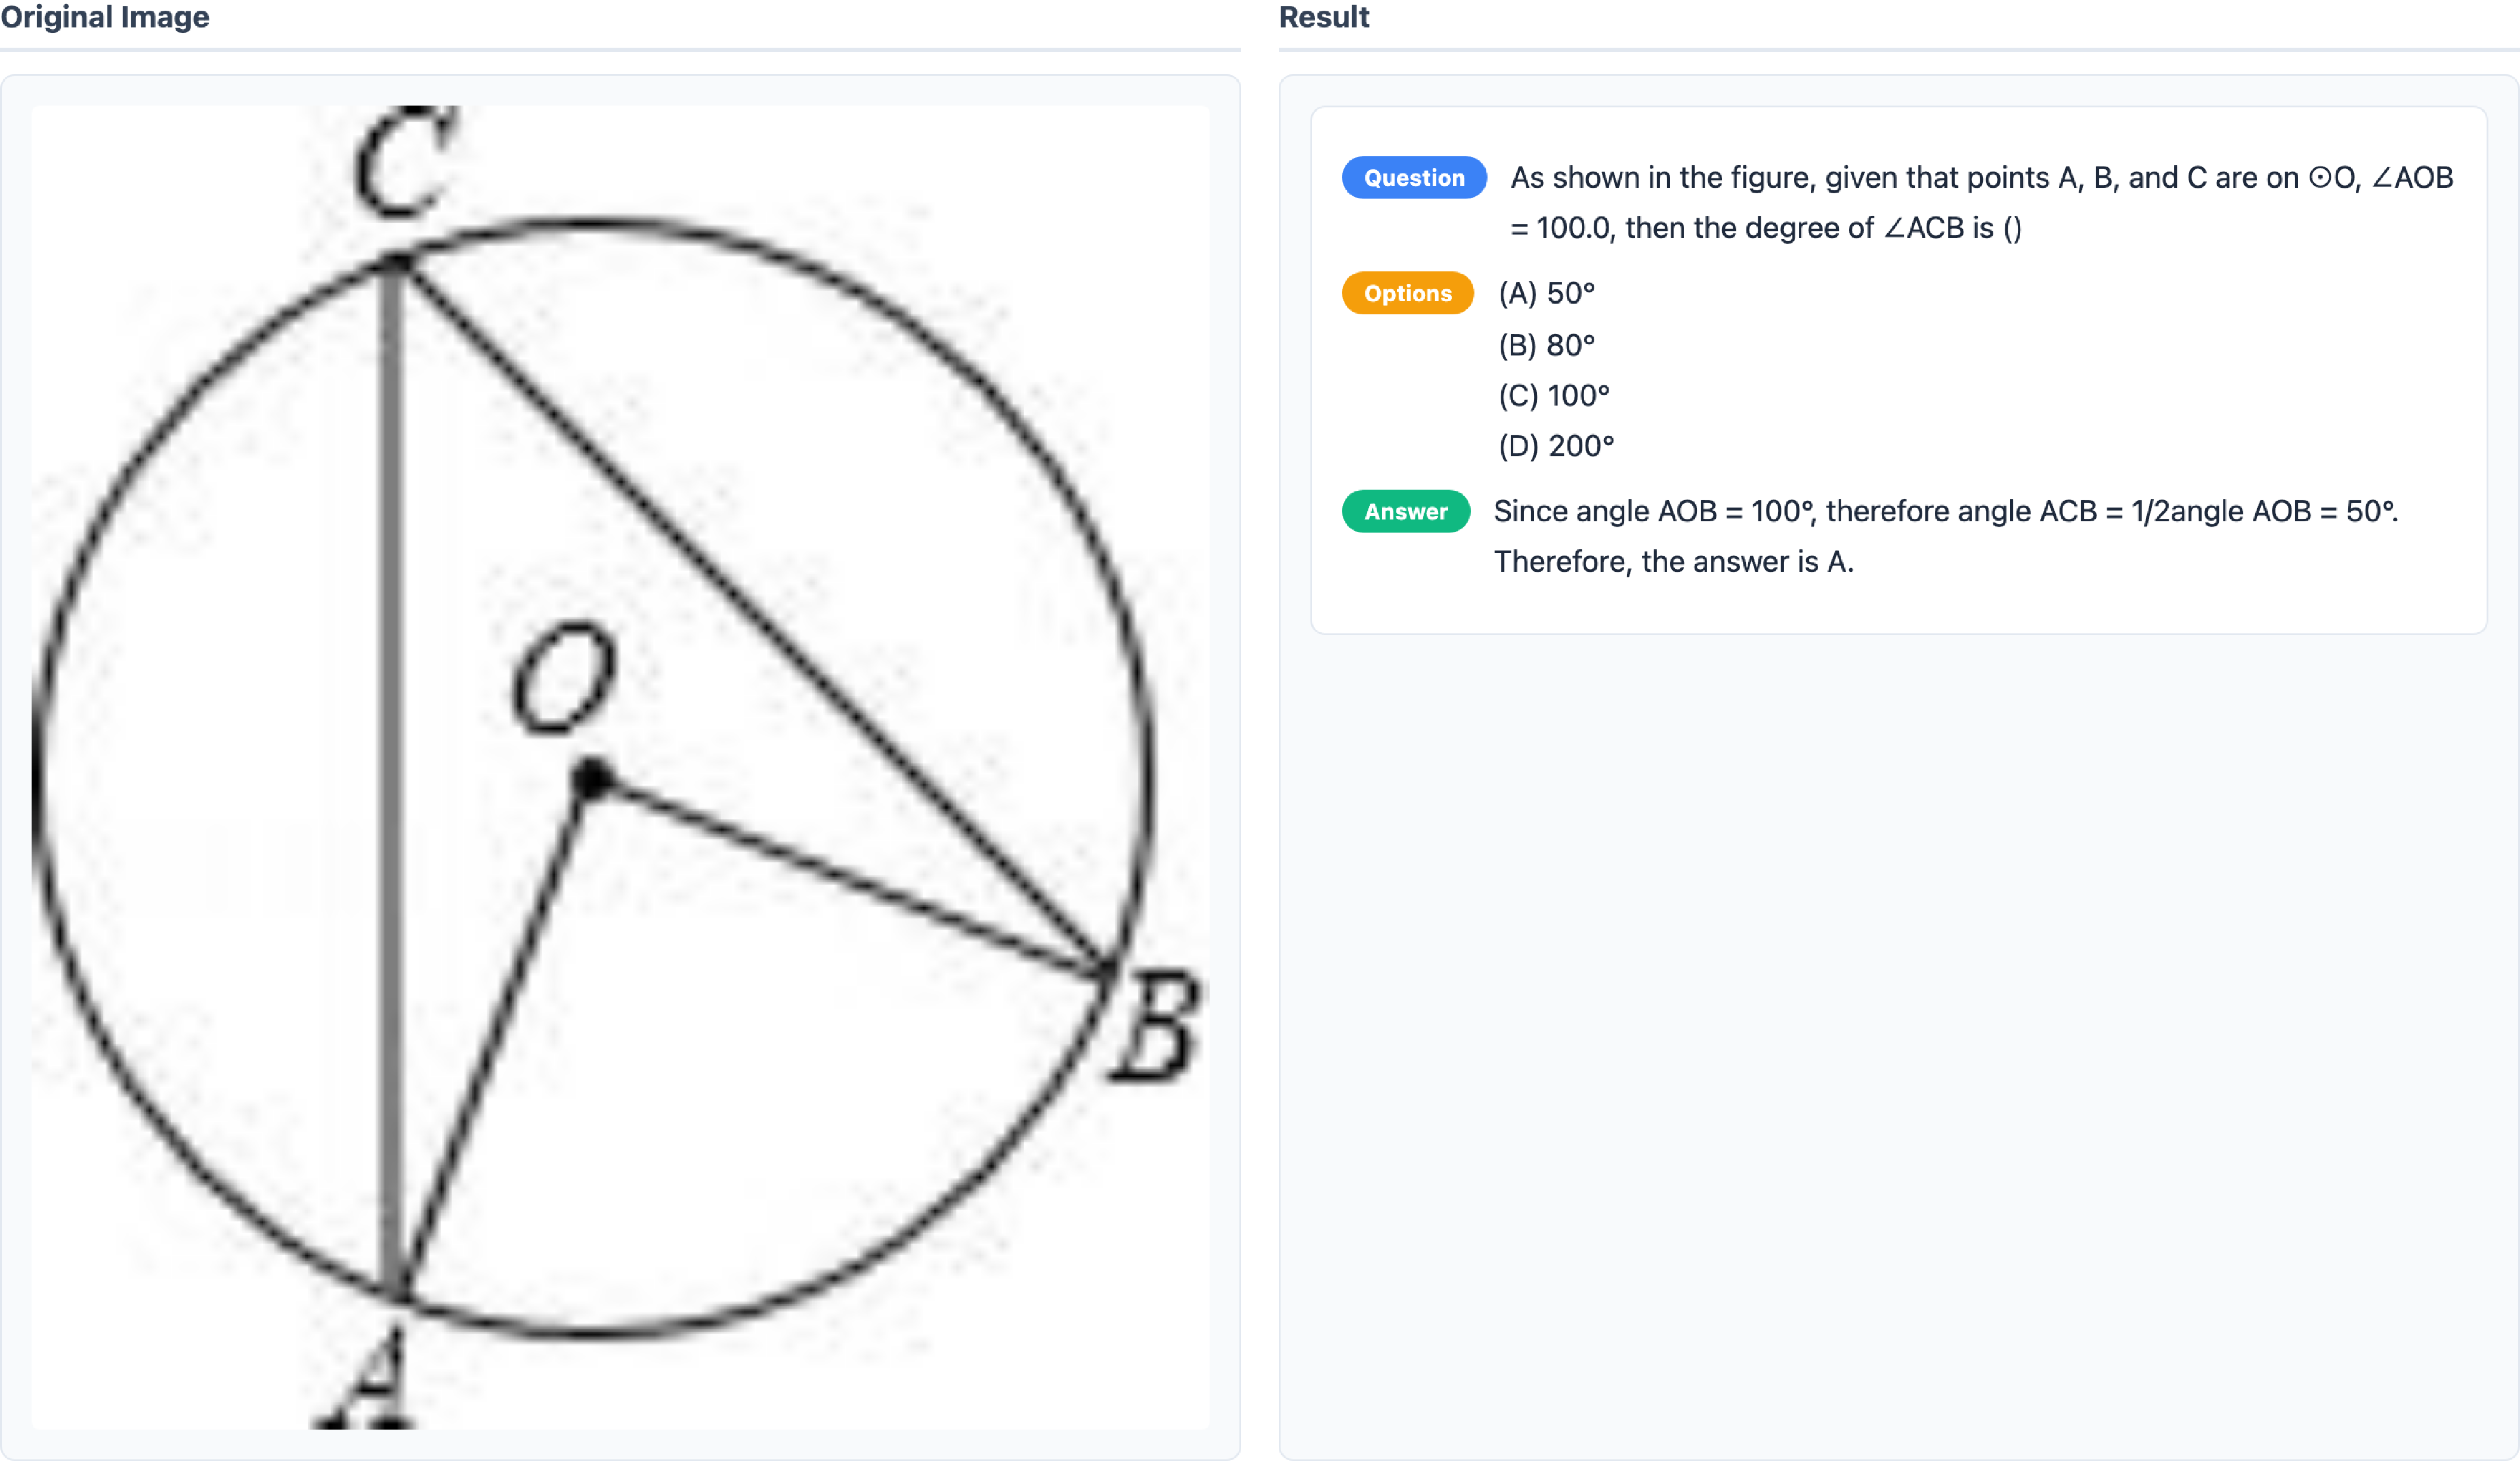
\includegraphics[width=\textwidth]{figures/visualization_results_mathvista.pdf}
    \caption{Visualization results of the MathVista task. The challenge is jointly interpreting the geometric figure and applying mathematical reasoning to derive the correct answer.}
    \label{fig:visualization_results_mathvista}
\end{figure*}

\begin{figure*}[htbp]
    \centering
    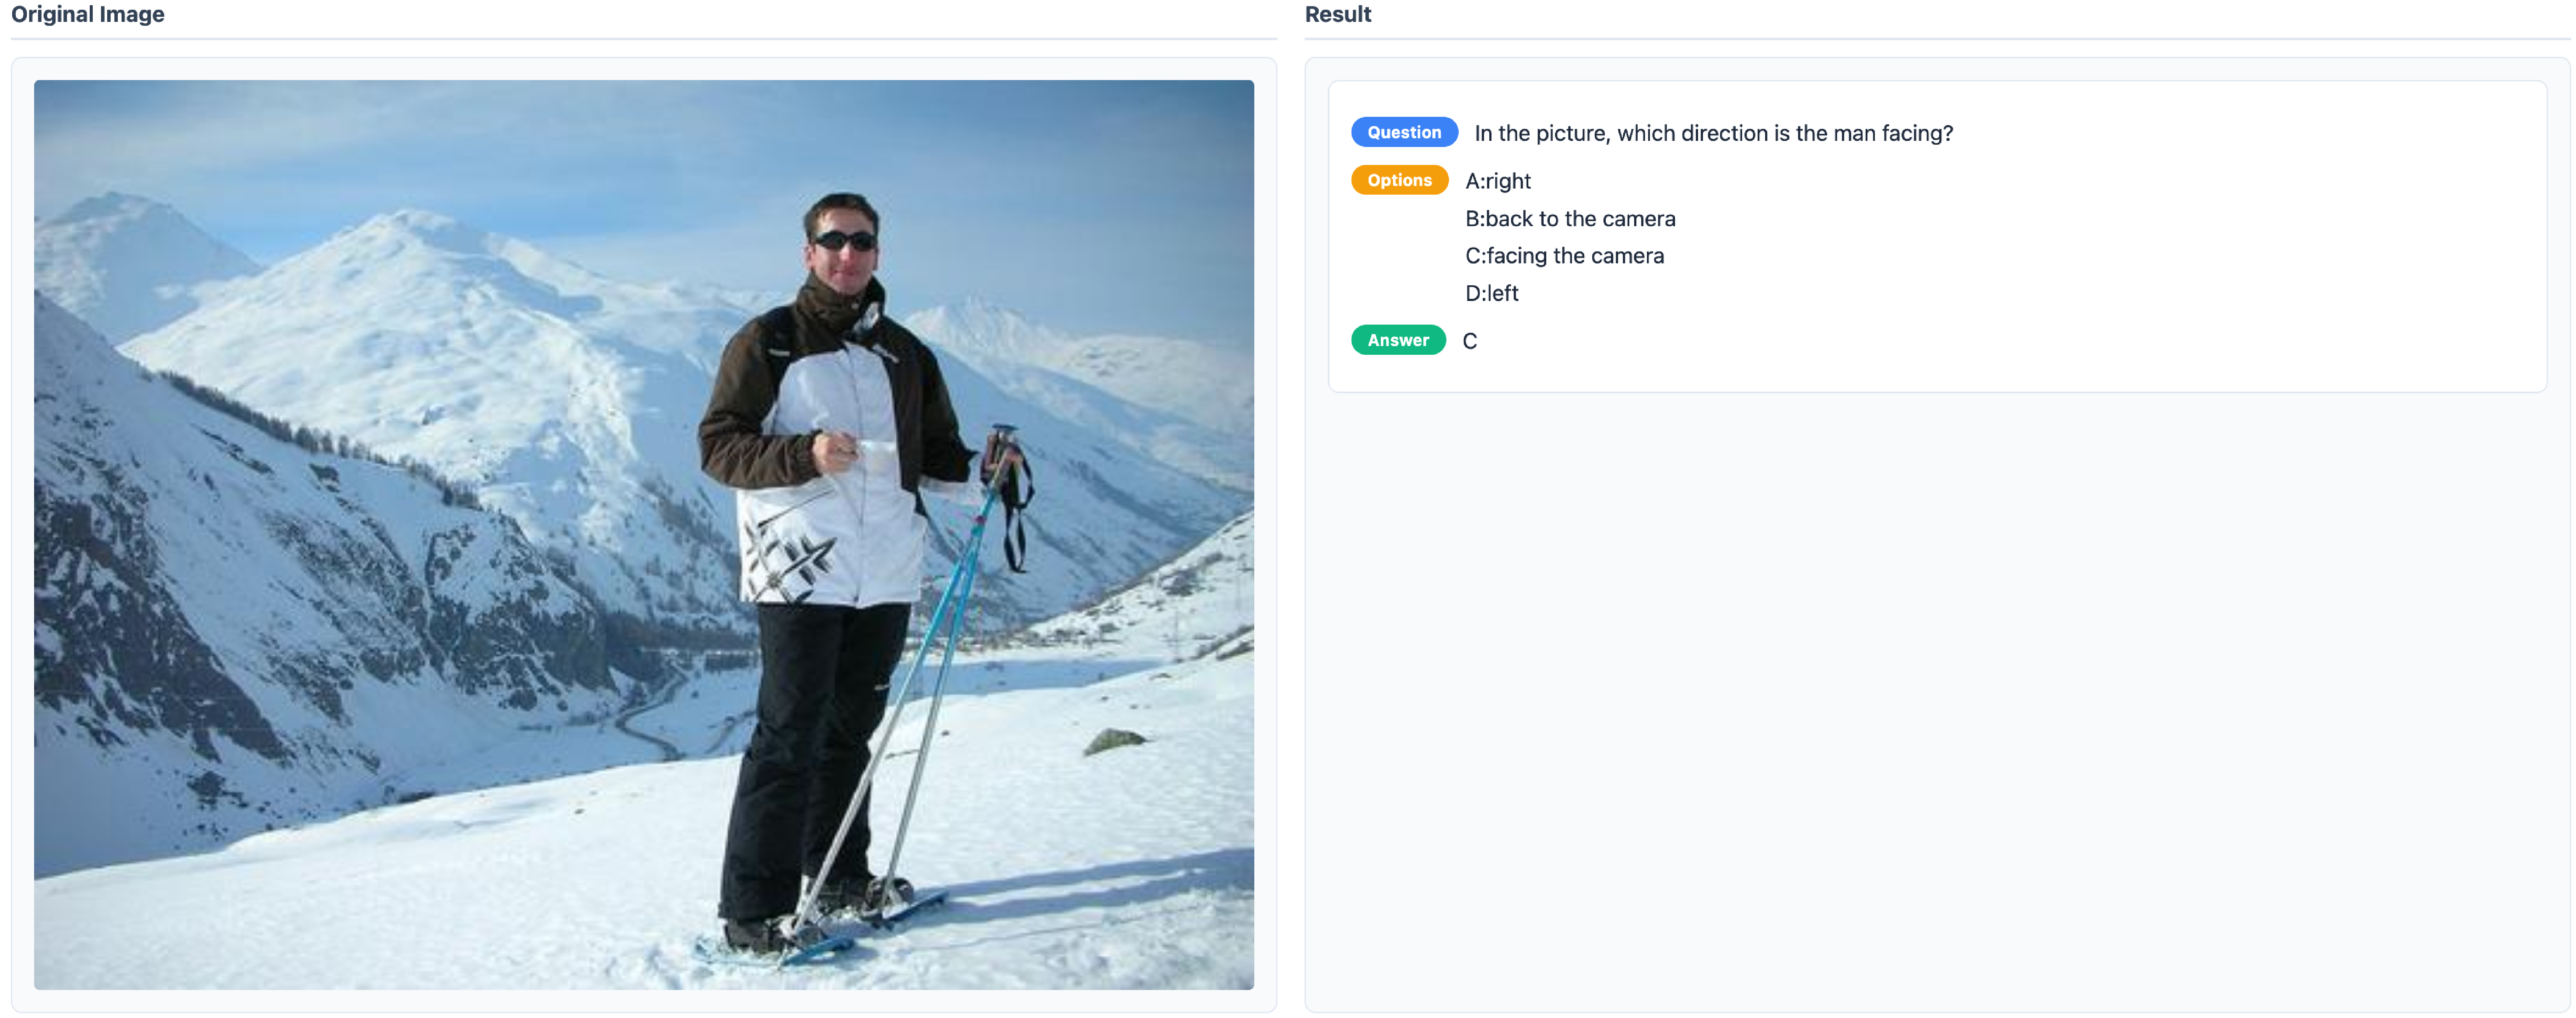
\includegraphics[width=\textwidth]{figures/visualization_results_mmbench.pdf}
    \caption{Visualization results of the MMBench task. The difficulty lies in fine-grained spatial perception and commonsense reasoning to determine the subject's orientation within a natural scene.}
    \label{fig:visualization_results_mmbench}
\end{figure*}